\def \sectionauthors {Samuel Bleiner}
\subsection{Einleitung}
Der Teil der Kennzeichenerkennung beschäftigt sich damit, aus aufgenommenen Fotos der einfahrenden und ausfahrenden Fahrzeuge, 
das Kennzeichen auszulesen und dieses an die Datenbank zu senden. Dies wird benötigt um damit es möglich ist zu bestimmen welches 
Fahrzeug sich im Moment auf dem Parkplatz befindet. Zudem kann dadurch jedes Fahrzeug eindeutig identifiziert werden, da das Kennzeichen 
einzigartig sein muss.  In Zusammenhang mit der Datenbankverwaltung können so auch bestimmte Kennzeichen definiert werden, welche anders 
behandelt werden als andere Kennzeichen. Ein Beispiel dafür wäre kostenloses Parken für den Parkplatzbesitzer oder auch gesperrte Kennzeichen, 
bei welchen der Parkplatzbetreiber eine Benachrichtigung bekommt, wenn sich diese auf dem Parkplatz befinden. Die Verbindung zur Datenbank 
erfolgt über eine eigene API, mit welcher die Daten schnell und einfach übertragen werden können. Um das Programm für die Kennzeichenerkennung 
zu realisieren werden sowohl bewährte Bildverarbeitungsalgorithmen eingesetzt als auch Neuronale Netze, welche sich in den Bereich des 
Maschinellen Lernens einordnen lassen, wodurch die Genauigkeit gesteigert werden kann. Zusätzlich wird für das komplette Modul ein Gehäuse 
gefertigt in welchem die Elektronik fest verbaut werden kann und trotzdem die Möglichkeit zu weiteren Verbesserungen ermöglicht.

\subsection{Anforderungen}
Das Modul für die Kennzeichenerkennung muss einige Anforderungen erfüllen, um für seinen Einsatzzweck bestmöglich geeignet zu sein.\\

Als erstes muss die Software einige Anforderungen erfüllen. Sie muss eine hohe Genauigkeit erreichen, um in möglichst jedem einzelnen Fall 
ein korrektes Ergebnis zu liefern. Um diese Genauigkeit zu erreichen werden mehrere Modell für Maschinelles Lernen verwendet, mit welchen 
eine bessere Genauigkeit als mit anderen Methoden erreicht werden kann. Die Geschwindigkeit ist hingegen ein nicht ganz so wichtiger Punkt, 
da Fahrzeuge für eine erfolgreiche Erkennung nicht zu schnell fahren dürfen, um eine passende Fotoaufnahme zu ermöglichen. Dadurch wird der 
Zeitintervall zwischen den Fahrzeugen erhöht, weswegen der Fokus bei der Software nahezu vollständig auf die Genauigkeit gelegt werden kann 
und die Geschwindigkeit bis zu einem gewissen Punkt vernachlässigt werden kann. Das bedeutet, dass die Software für einen Durchlauf mehrere 
Sekunden benötigen darf, ohne dadurch auch nur annähernd die Anwendung zu behindern. Außerdem muss die Leistung eines Raspberry Pi 4 2GB für 
die Software ausreichen, da dieser für das Modul verwendet wird.\\

Als nächstes kommt der Auslöser für die Fotoaufnahme. Dieser muss so auslösen, dass das Fahrzeug sich in einer Position vor der Kamera befindet 
und muss unabhängig von der Art des Fahrzeuges, also egal ob es ein kleines Auto oder ein großer SUV ist, ungefähr an der gleichen Position auslösen. 
In dieser Applikation wird dafür ein manueller Button verwendet, aber in einer möglichen Verbesserung wäre es sinnvoll diesen durch eine Lichtschranke oder ähnliches zu ersetzen.\\

Der letzte Punkt ist dann noch das Gehäuse. Dieses muss stabil genug sein, um fest verbaut zu werden, Zugang zu den wichtigsten Anschlüssen 
bieten und eine Halterung für die Kamera sollte auch integriert sein. Um für die Entwicklung ein geeignetes Gehäuse zu entwickeln wurde hier ein 
Gehäuse mit einem 3D-Drucker erstellt. Das Gehäuse wird von oben und unten verschraubt und bietet die Möglichkeit die Kamera mit Schrauben zu sichern. 
Die Anschlüsse für die Stromversorgung, die USB-Ports, die HDMI-Ports, den Ethernet-Anschluss und die GPIO-Pins sind zugänglich damit es auch weiterhin 
möglich ist damit zu arbeiten, auch wenn kleine Änderungen durchgeführt werden. Zudem ist es dadurch auch möglich zu Test- und Entwicklungszwecken einen Bildschirm anzuschließen.

\subsection{Bildverarbeitung}

\subsubsection{Einleitung}
Die Bildverarbeitung ist ein zentrales Thema in dieser Applikation für Kennzeichenerkennung. 
Sie wird für die Zeichensegmentierung verwendet, sowie für die Vorbereitung von Bildern für 
andere Algorithmen. Im Folgenden werden die verwendeten Bildverarbeitungsfunktionen aufgelistet 
und deren Funktionsweise erläutert.

\subsubsection{Bilaterale Filterung}
Bilaterale Filterung ist eine Methode für eine kantenerhaltende Weichzeichnung eines Bildes.\\

Bei der Berechnung für den Farbwert des Ausgabepixels werden die benachbarten Pixel nicht nur 
mit ihrer Entfernung gewichtet, sondern auch mit ihrem eigenen Farbwert. Dadurch können einzelne 
farbliche Ausreißer herausgefiltert werden. Dies ist vor allem in der Bildverarbeitung wichtig, 
da dadurch die wichtigen Eigenschaften eines Bildes, wie zum Beispiel Kanten, erhalten bleiben 
und verarbeitet werden können, aber einzelne abweichende Pixel herausgefiltert werden wodurch 
unnötige Informationen entfernt werden.\\ 

\begin{figure}[htbp]
    \centering
    \begin{minipage}[t]{0.45\linewidth}
        \centering
        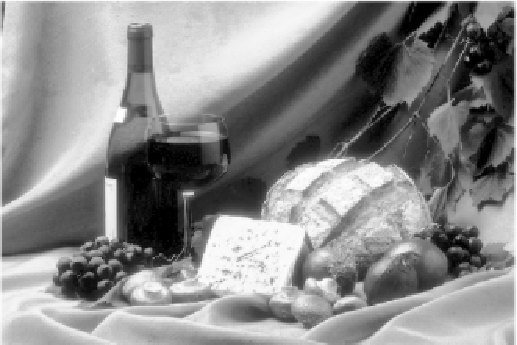
\includegraphics[width=\linewidth]{kennzeichenerkennung/vorBilateral.pdf}
        \caption{Vor Bilateraler Filterung}
        \label{vorBi}
    \end{minipage}
    \hfill
    \begin{minipage}[t]{0.45\linewidth}
        \centering
        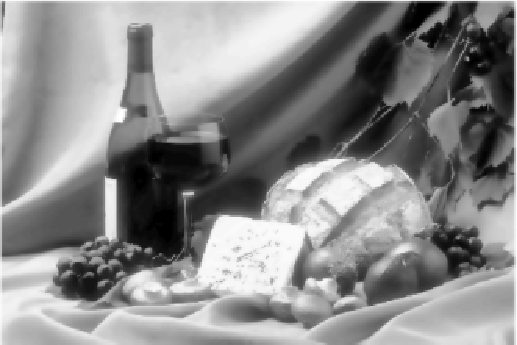
\includegraphics[width=\linewidth]{kennzeichenerkennung/nachBilateral.pdf}
        \caption{Nach Bilateraler Filterung}
        \label{nachBi}
    \end{minipage}
\end{figure}

In Abbildung \ref{vorBi} kann man ein Bild von verschieden Lebensmitteln sehen. Wenn man genau hinsieht 
erkennt man vor allem bei den Blättern im Hintergrund und beim Brot viele detailreiche Texturen. 
Diese Texturen haben keine wichtige Texturen und sind deswegen unnötig. Um die Bildverarbeitung zu 
vereinfachen wendet man deswegen die bilaterale Filterung auf dieses Bild an, um diese detailreichen 
Texturen zu vereinfachen. In Abbildung \ref{nachBi} sieht man das Bild nach der bilateralen Filterung. 
Wenn man hier dann wieder genauer auf die Blätter und das Brot sieht, erkennt man, dass die 
detailreichen Texturen weichgezeichnet wurden, aber die Kanten sind genauso gut erkennbar wie vor der Filterung.

\subsubsection{Thresholding}
Das Thresholding oder auch Schwellenwertverfahren wird in der Bildverarbeitung verwendet, um Bilder zu segmentieren. 
Aus einem Graubild kann dadurch ein Binäres Bild erzeugt werden.\\ 

Bei diesem Verfahren wird ein bestimmter Schwellwert (En.: Threshold) definiert, welcher mit den Grauwerten der einzelnen 
Pixel des Bildes verglichen wird. Wenn der Grauwert den Schwellwert überschreitet, wird dieser durch einen weißen Pixel 
ersetzt und wenn der Grauwert kleiner als der Schwellwert ist, wird dieser durch einen schwarzen Pixel ersetzt. 
Dadurch erhält man ein Bild welches nur noch zwei Farben hat, Schwarz und Weiß. Dies wird deswegen eingesetzt, 
da dadurch viele Bildverarbeitungsalgorithmen schneller arbeiten und die Effizienz gesteigert wird.\\

\begin{figure}[htbp]
    \centering
    \begin{minipage}[t]{0.45\linewidth}
        \centering
        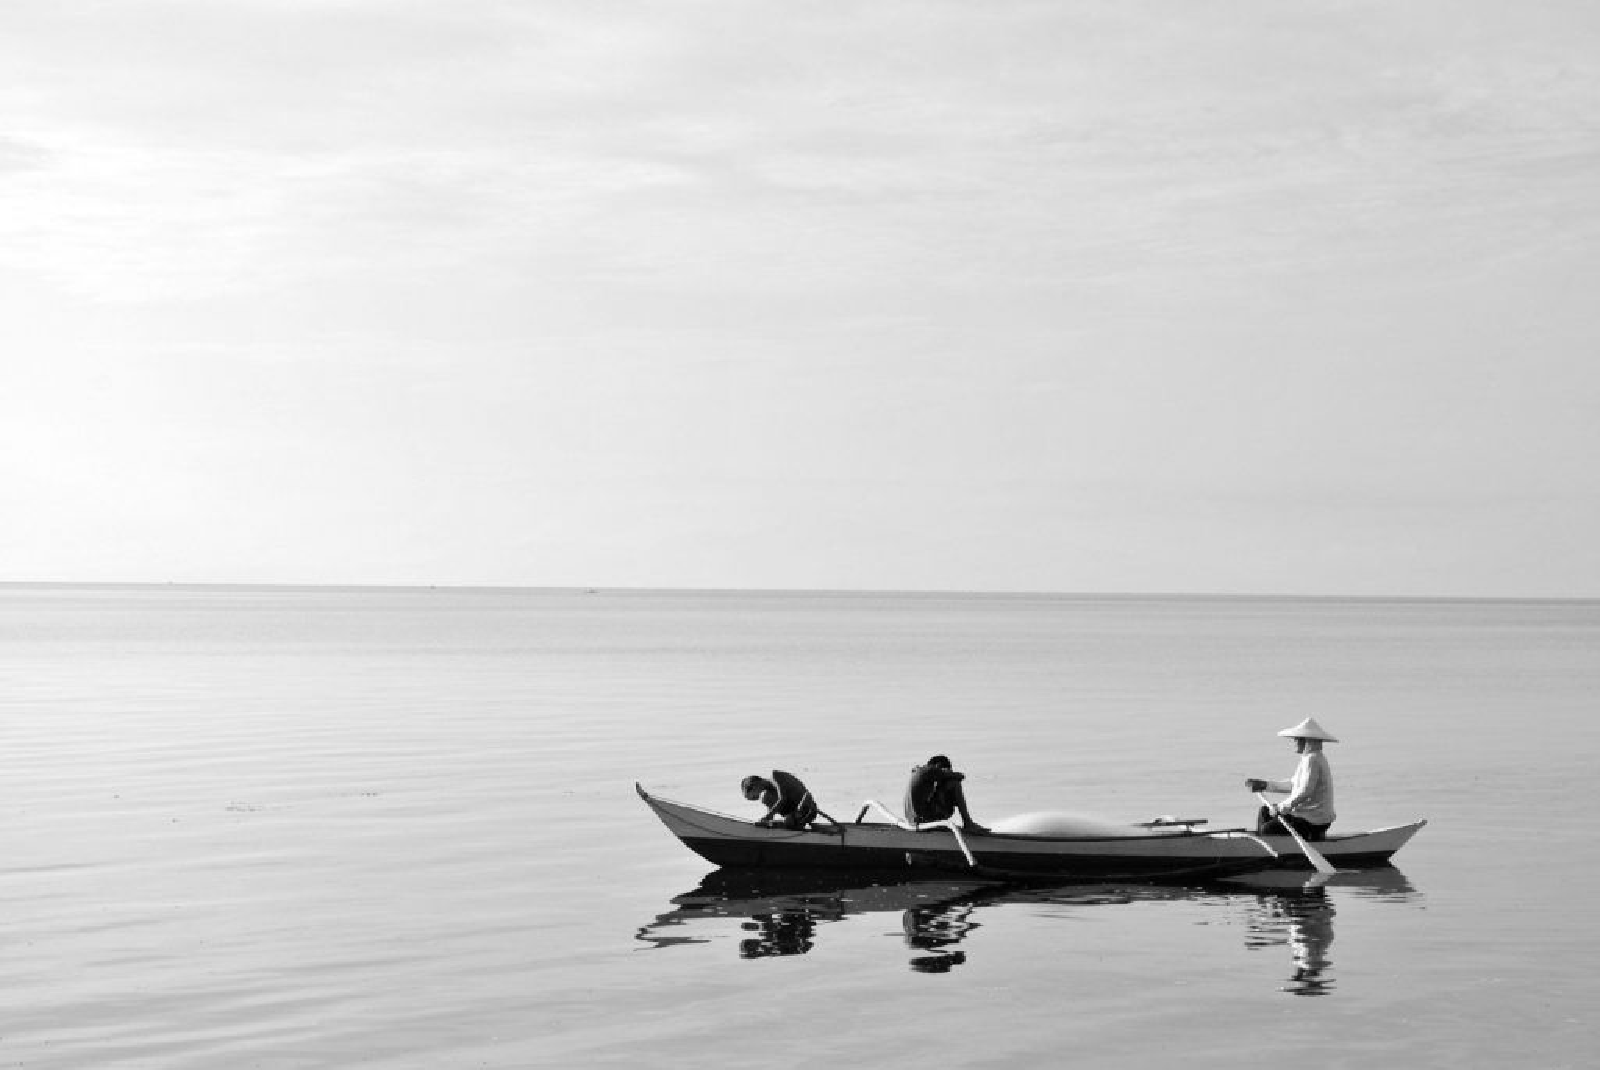
\includegraphics[width=\linewidth]{kennzeichenerkennung/graustufen.pdf}
        \caption{Graustufenbild}
        \label{graypic}
    \end{minipage}
    \hfill
    \begin{minipage}[t]{0.45\linewidth}
        \centering
        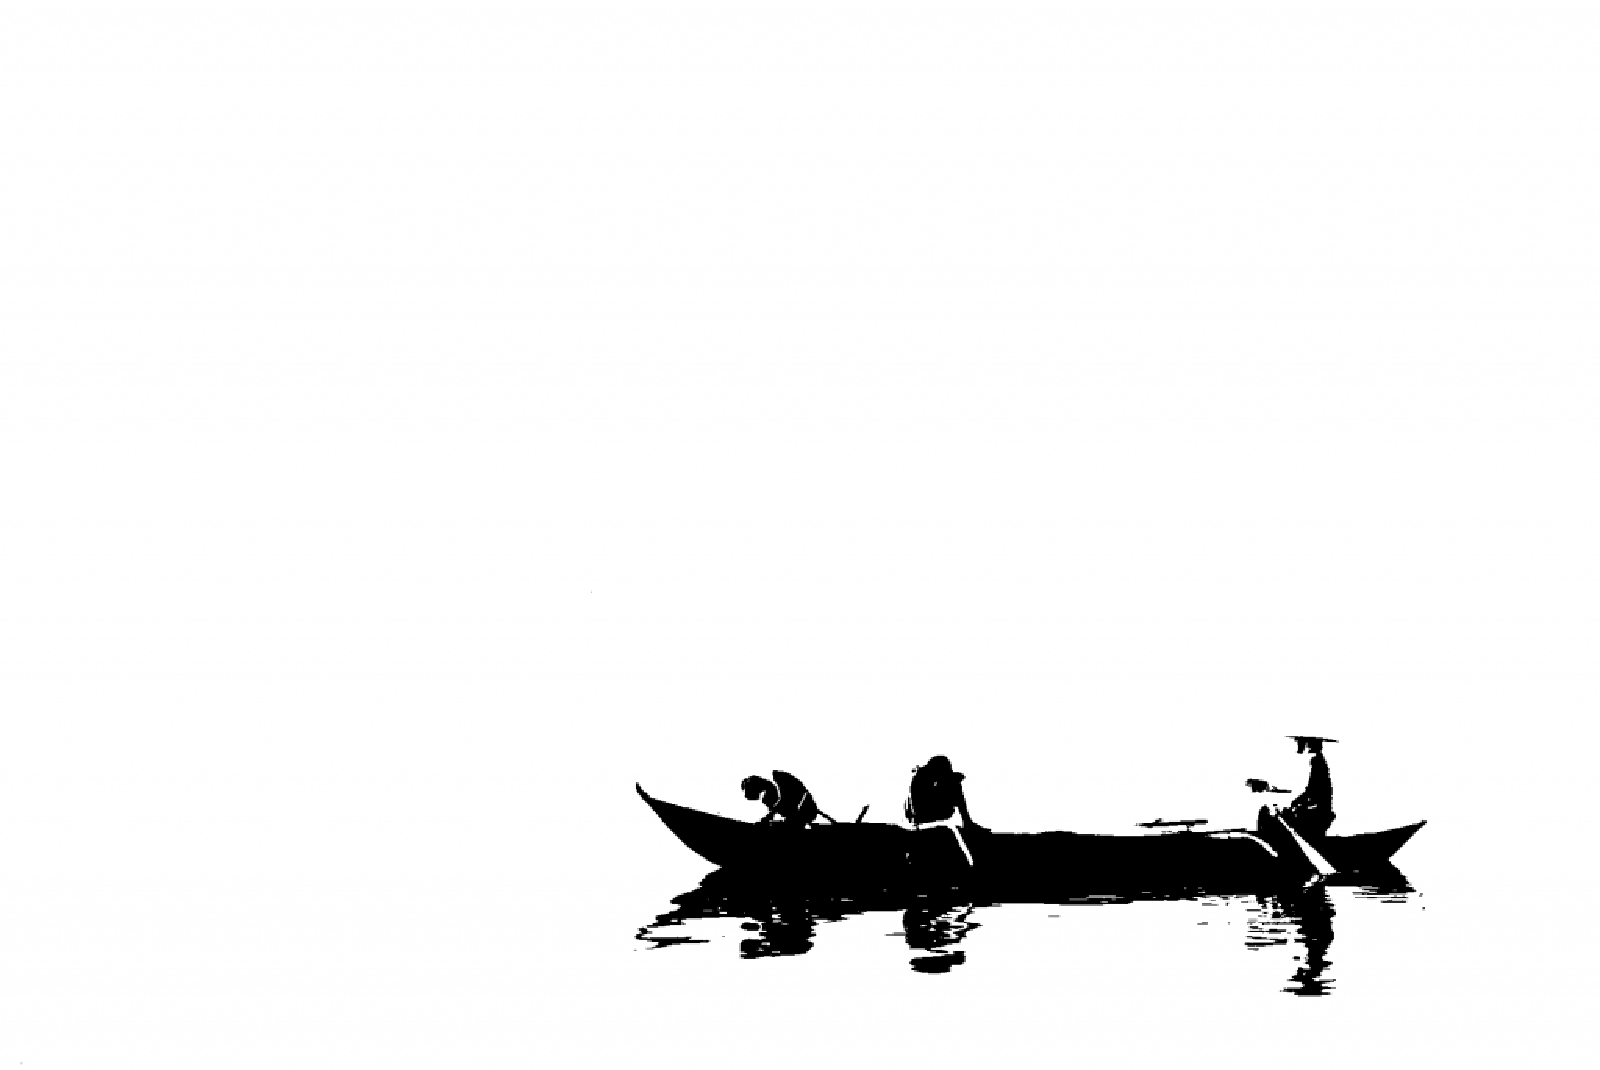
\includegraphics[width=\linewidth]{kennzeichenerkennung/binary.pdf}
        \caption{Binäres Bild nach Thresholding}
        \label{binarypic}
    \end{minipage}
\end{figure}

In Abbildung \ref{graypic} sieht man ein solches Graubild welches nur verschieden Graustufen aufweist. In Abbildung \ref{binarypic} sieht man das 
Bild nach dem Thresholding. Hier kann man nur noch das Boot mit den Menschen erkennen. Dies ist nicht nur für schnellere 
Bildverarbeitungsalgorithmen wichtig, sondern wird auch zur Objekterkennung in Bildern verwendet.\\

Um den Schwellwert zu bestimmen kann man diesen entweder variieren bis das gewünschte Ergebnis erscheint oder man 
verwendet Methoden, welche den Schwellwert automatisch bestimmen. Eine der bekanntesten Methoden zur Schwellwertbestimmung 
ist die Methode von Otsu\footnote{Benannt nach Nobuyuki Otsu}, welche mit dem Schwellenwert die Pixel in Vordergrund und Hintergrund unterteilt.

\subsubsection{Erosion}
Erosion ist eine Funktion der Bildverarbeitung und ist in die morphologische Bildverarbeitung einzuordnen. Diese beschäftigt 
sich primär mit der Verarbeitung von binären Bildern, welche man nach Thresholding erhält.\\

Erosion benötigt zwei Eingaben, das binäre Bild und einen Kernel. Der Kernel ist dabei die Angabe, nach welcher die Erosion 
durchgeführt wird. Der Kernel ist auch eine binäre Struktur, welche über jeden einzelnen Pixel des binären Bildes geschoben 
wird. Wenn der Kernel komplett mit dem binären Bild übereinstimmt, behält dieser Pixel seinen Wert und ansonsten wird er 
invertiert. Dabei muss jedoch darauf geachtet werden, dass die Polarität des binären Bildes und des Kernels übereinstimmt, 
da sonst die Erosion nicht richtig funktioniert. Als Resultat erhält man danach ein deutlicheres Bild bei welchem einzelne 
Pixelfehler herausgefiltert wurden und die Konturen besser erkennbar sind.\\

\begin{figure}[htbp]
    \centering
    \begin{minipage}[t]{0.45\linewidth}
        \centering
        
\includegraphics[width=\linewidth]{kennzeichenerkennung/kennBinary.pdf}
        \caption{Binäres Bild nach Thresholding}
        \label{kennbinpic}
    \end{minipage}
    \hfill
    \begin{minipage}[t]{0.45\linewidth}
        \centering
        
\includegraphics[width=\linewidth]{kennzeichenerkennung/kennErosion.pdf}
        \caption{Nach Erosion}
        \label{eropic}
    \end{minipage}
\end{figure}

In Abbildung \ref{kennbinpic} und \ref{eropic} sieht man die Anwendung der Erosion. Die Konturen der einzelnen Zeichen im Kennzeichen sind in Abbildung 
\ref{eropic} nach der Erosion deutlicher erkennbar als davor.

\subsubsection{Farbraum}
Der Farbraum eines Bildes enthält alle möglichen Farben eines Farbmodells. Das Farbmodell beschreibt dabei die Parameter, aus 
welchen die einzelnen Farben gebildet werden. Dies ist in der Bildverarbeitung relevant, da verschiedene Funktionen der 
Bildverarbeitung, unterschiedliche Farbräume verwenden und dieser deswegen korrekt eingestellt werden muss.\\

In dieser spezifischen Applikation werden die folgenden Farbräume verwendet:

\paragraph{RGB}\mbox{}\\
RGB ist einer der häufigsten und bekanntesten Farbräume. Er basiert auf den drei Grundfarben Rot, Grün und Blau und wird vor 
allem bei Bildschirmen und in der Fotografie genutzt. Die Farben setzen sich in diesem Modell aus dem jeweiligen Rot-, Grün- 
und Blauanteil der einzelnen Pixel zusammen.

\paragraph{Graustufen}\mbox{}\\
Bei einem Graustufen-Bild, zu sehen in Abbildung 3, hat jeder Pixel einen Wert von 0 bis 255. Diese Werte erstrecken sich also 
von Schwarz bis Weiß und dazwischen liegen verschiedene Grautöne. Dieser Farbraum wird in der Bildverarbeitung häufig verwendet, 
da Konturen einfacher erkennbar sind und es nur einen Parameter gibt, welcher verarbeitet werden muss, wodurch die Effizienz 
diverser Algorithmen gesteigert werden kann. Zudem wird dieser Farbraum auch oft in Verbindung mit Thresholding verwendet.

\paragraph{BGR}\mbox{}\\
Der BGR ist ein relativ unbekannter und wenig verwendeter Farbraum, da er sehr ähnlich zum RGB-Farbraum ist. Der einzige 
Unterschied zwischen diesen beiden liegt in der Anordnung der Parameter. Bei BGR sind die Parameter spiegelverkehrt zu RGB, 
das heißt es kommt zuerst der Blauanteil, dann der Grünanteil und zum Schluss der Rotanteil. Insgesamt ergibt dies für die 
einzelnen Pixel zwar die gleichen Farben, aber die Funktionen der Bildverarbeitung müssen trotzdem das Bild im passenden 
Farbraum erhalten. So verwendet zum Beispiel die Funktion „imread“ von OpenCV den BGR-Farbraum und die Funktion „im Show“ 
von Matplotlib verwendet den RGB-Farbraum. Wenn man diese Funktionen also nacheinander anwendet, muss dazwischen der Farbraum 
umgewandelt werden.

\subsubsection{Konturerkennung}
Die Konturerkennung ist eine wichtige Funktion in der Bildverarbeitung mit welcher Objekte in einem Bild gefunden werden können. 
In dieser Applikation wird sie für die Zeichensegmentierung eingesetzt.\\

Die Konturerkennung wird hauptsächlich bei binären Bildern verwendet. Eine Kontur kann dabei wie im Folgenden definiert werden. 
Man überprüft jeden einzelnen Pixel und sieht nach, ob ein benachbarter Pixel einen anderen Farbwert aufweist. Falls dies 
zutrifft muss der zu prüfende Pixel zu einer Kontur gehören. Wenn dies auf mehrere zusammenhängende Pixel zutrifft, bedeutet 
das, dass diese zusammen eine Kontur bilden.\\

Die Funktion „findcontours“ von OpenCV, welche in dieser Applikation verwendet wird, ist eine Funktion für Konturerkennung 
und kann weiße Objekte auf einem schwarzen Hintergrund erkennen. Sie basiert auf dem Algorithmus von Suzuki von 
1985\footnote{Topological structural analysis of digitized binary images by border following} und 
liefert eine Liste mit allen Konturen. Die Konturen werden in der Liste als ein Array von Koordinaten abgespeichert.

\subsection{Kennzeichenerkennungsprogramm}

\subsubsection{Einleitung}
Die Software ist der wichtigste und größte Teil der Kennzeichenerkennung. Sie erhält ein Bild, in welchem ein Auto mit 
einem Kennzeichen enthalten ist und liefert am Ende dieses Kennzeichen und sendet dieses dann automatisch an die Datenbank. 
Die Software kann entweder über Bildverarbeitung oder mit Modellen für Maschinelles Lernen realisiert werden. Der erste Ansatz bei 
dieser Anwendung war mit klassischer Bildverarbeitung, welche aber nicht die gewünschte Genauigkeit erreicht hat, weswegen 
dann auf Maschinelles Lernen gewechselt wurde.

\subsubsection{Programmiersprache}
Die verwendete Programmiersprache für die Kennzeichenerkennung ist Python. Python ist eine höhere Programmiersprache, 
welche übersichtlich und leicht lesbar ist. Sie ist vor allem für Bildverarbeitung und Anwendungen mit Maschinellem Lernen gut geeignet, 
da es dafür hoch optimierte und effiziente Bibliotheken gibt wie zum Beispiel OpenCV, Numpy und Tensorflow. Dadurch ist Python 
für diese Anwendung besser geeignet als zum Beispiel C++. Dieses wäre zwar normalerweise effizienter, bietet aber weniger 
optimierte Bibliotheken in diesem Bereich, wodurch es hier weniger gut geeignet ist.

\subsubsection{Konzept}
Das Programm für die Kennzeichenerkennung basiert auf fünf Stufen. Die erste Stufe ist die Bildaufnahme, die zweite ist die 
Kennzeichenerfassung mittels Maschinellem Lernen, die dritte ist die Kennzeichensegmentierung mithilfe von Bildverarbeitung, 
die vierte ist die Zeichenerkennung mittels Maschinellem Lernen und die fünfte ist die Anbindung an die Datenbank.

\paragraph{Bildaufnahme}\mbox{}\\
Um ein Bild verarbeiten zu können und aus diesem ein Kennzeichen auslesen zu können, muss zuerst ein Bild vorliegen. 
Dieses wird über den RaspberryPi mit der RaspberryPi-Kamera aufgenommen. Um das Bild aufzunehmen, muss einfach ein Auslöser 
aktiviert werden und dann wird das Bild aufgenommen und im richtigen Ordner abgespeichert. Zuvor wird noch überprüft ob 
sich in diesem Ordner bereits ein Bild befindet und falls eines vorhanden ist wird es gelöscht. Dadurch werden mögliche Fehler 
durch mehrere Bilder verhindert.

\paragraph{Kennzeichenerfassung}\mbox{}\\
Die Kennzeichenerfassung hat die Aufgabe, das Kennzeichen im Eingabebild zu lokalisieren. Dies geschieht mittels Maschinellem Lernen 
mit dem Modul WPOD-NET von Sérgio Montazolli Silva und Cláudio Rosita Jung\footnote{License Plate Detection and Recognition in Unconstrained Scenarios}. Dieses verwendet zuerst das Modul YOLOv2 welches zur 
Echtzeitobjekterkennung verwendet werden kann und in dieser Anwendung zur Erkennung von Fahrzeugen verwendet wird. Danach werden 
die Koordinaten des Kennzeichens ermittelt und dieses aus dem Bild ausgeschnitten und abgespeichert.

\paragraph{Kennzeichensegmentierung}\mbox{}\\
Die Kennzeichensegmentierung hat das Ziel die einzelnen Zeichen im Kennzeichen zu separieren und so zu vorbereiten, dass die 
darauffolgende Zeichenerkennung damit arbeiten kann. Dazu wird das Bild mit dem Kennzeichen zuerst in Graustufen konvertiert, 
dann mit einem bilateralen Filter gefiltert, mit Thresholding in ein binäres Bild umgewandelt und anschließend mittels Erosion 
besser erkennbar gemacht. Danach werden im verarbeiteten Bild die Konturen gesucht, sortiert und anhand dieser die einzelnen Zeichen herausgefiltert.

\paragraph{Zeichenerkennung}\mbox{}\\
Die letzte Stufe der Kennzeichenerkennung ist die Zeichenerkennung. In dieser werden die einzelnen Zeichen erkannt und als Text 
abgespeichert. Dies funktioniert über eine eigenes Neuronales Netz basierend auf MobileNetV2\footnote{Neuronales Netz für Computer Vision}, welches mit einem Datensatz von 
über 35 000 Bildern auf die Erkennung von Zeichen aus Bildern trainiert wurde.

\paragraph{Anbindung an Datenbank}\mbox{}\\
Nachdem das Kennzeichen als Text abgespeichert wurde, muss diese Information in die Datenbank übergeben werden. Dazu wird die 
eigene API angewandt, welcher man diese Informationen übergeben muss und als Rückgabe die Information bekommt, ob sich das 
Fahrzeug nun innerhalb oder außerhalb des Parkplatzes befindet.

\subsubsection{Ablauf}

\begin{figure}[H]
    \centering
    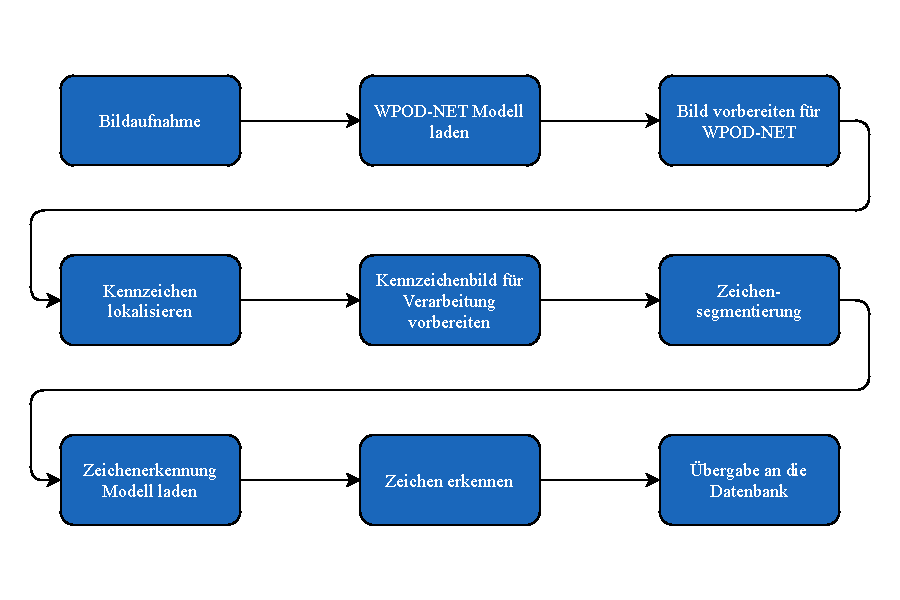
\includegraphics[width=0.9\linewidth]{kennzeichenerkennung/Programmablauf.pdf}
    \caption{Ablaufdiagramm der Kennzeichenerkennung}
\end{figure}

Im oberen Diagramm ist der Ablauf des Programms angegeben. Zuerst wird mit einem Button der Auslöser betätigt und damit das 
Foto aufgenommen. Dann wird das erste Modell für Maschinelles Lernen für die Kennzeichenerkennung „WPOD-NET“\footnote{Modell für Maschinelles Lernen für Kennzeichenerfassung} geladen. Bevor das 
Bild diesem Modell übergeben werden kann, muss es noch angepasst werden damit das Modell damit arbeiten kann. Danach kann 
damit das Kennzeichen im Bild lokalisiert werden. Im Anschluss wird dieses Kennzeichenbild mit mehreren Bildverarbeitungsalgorithmen 
verarbeitet, um dann die einzelnen Zeichen zu segmentieren. Danach kann dann das Modell für die Zeichenerkennung geladen 
werden und dieses dann auch angewendet werden, um das Ergebnis zu erhalten. Dieses Ergebnis wird dann noch mit einer API an die Datenbank übergeben.

\subsubsection{Verwendete Libraries}

\paragraph{Versionsübersicht der verwendeten Libraries}\mbox{}\\
Im Folgenden werden die verwendeten Versionen der benötigten Libraries aufgelistet, um das Programm zu starten. Dies wird noch einmal 
unterteilt in die Versionen, welche auf Windows 10 benötigt werden und jene auf Raspbian\footnote{Raspbian ist ein Unix-basiertes Betriebssystem für den Raspberry Pi}, da auf Raspbian manche Versionen noch 
nicht verfügbar sind, neuere und verbesserte Versionen verfügbar sind oder manche Versionen nur auf komplizierten Umwegen installierbar sind.

Windows:

\begin{itemize}
    \item h5py = 2.10.0
    \item imutils = 0.5.3
    \item Keras = 2.4.3
    \item matplotlib = 3.3.2
    \item notebook = 6.1.5
    \item numpy = 1.18.5
    \item opencv-python = 4.4.0.44
    \item scikit-learn = 0.23.2
    \item tensorflow = 2.3.1
    \item requests = 2.24.0
\end{itemize}

Raspbian:

\begin{itemize}
    \item h5py = 2.10.0
    \item imutils = 0.5.3
    \item Keras = 2.4.3
    \item matplotlib = 3.3.3
    \item notebook = 6.1.5
    \item numpy = 1.19.4
    \item opencv-python = 4.4.0.46
    \item scikit-learn = 0.24.0
    \item tensorflow = 2.4.0
    \item requests = 2.21.0
\end{itemize}

\paragraph{Jupyter Notebook}\mbox{}\\
Jupyter Notebook ist eine nützliche Erweiterung für Python, wenn es um den Bereich der Daten-Visualisierung und Maschinelles Lernen geht. 
Sie ist eine Unteranwendung des Open-Source Projektes „Project Jupyter“, welches von großen Partnern wie Microsoft und Google unterstützt 
und verwendet wird. Mit Jupyter Notebook ist es möglich in einer Web-Anwendung ein Live-Script abzuarbeiten und in Kombination mit Matplotlib 
die Daten visuell darzustellen, abzuspeichern und zu überwachen. Im Gegensatz zur direkten Darstellung in der Entwicklungsumgebung, wird 
der letzte Durchgang des Scripts, inklusive aller Bilder und Grafiken gespeichert. Zudem ist es auch hervorragend für das Training und 
die dazugehörende Überwachung von Modulen für Maschinelles Lernen geeignet. Außerdem bietet Jupyter Notebook noch die Möglichkeit mehrere Scripts 
parallel abzuarbeiten und diese individuell zu überwachen. In dieser Applikation wird es für ein solches Training und für die anschauliche 
Visualisierung von Daten genutzt.\\

Die Installation von Jupyter Notebook ist simpel, da man es einfach über pip\footnote{Paketverwaltungsprogramm für Python} mit dem folgenden Befehl installieren kann:

\begin{listing}[H]
    \begin{minted}{bash}
    pip install notebook
    \end{minted}
    \caption{PIP Installation von Jupyter Notebook}
\end{listing}

Um das Jupyter Notebook aufzurufen muss im Terminal „jupyter notebook“ eingegeben werden und dann öffnet sich automatisch die Web-Applikation. 
Danach hat man Zugriff auf komplette Dateistruktur des eigenen Projektes und kann die einzelnen Python-Scripts starten. Dabei ist zu beachten, 
dass man keine gewöhnliche .py-Datei benötigt, sondern eine .ipynb-Datei benötigt, wozu man einfach eine Kopie des normalen Scripts erstellt und die Dateiendung ändert.

\paragraph{Numpy}\mbox{}\\
Numpy ist eine weit verbreitete Library für Python, welche sich mit der Berechnung und Verarbeitung von mehrdimensionalen Arrays beschäftigt. 
Damit können komplexe Berechnungen und Algorithmen oft effizienter verarbeitet werden, wobei aber beachtet werden muss, dass der Code an die 
mehrdimensionalen Arrays angepasst werden muss. Numpy selbst ist auch eine Voraussetzung für OpenCV, welches Numpy-Arrays verwendet, um Bilder zu verarbeiten. 
Dazu werden 3-dimensionale Arrays verwendet, wodurch die Verarbeitung dieser Bilder und die Bildverarbeitungsalgorithmen schneller sind. In dieser 
Applikation wird Numpy in Zusammenarbeit mit OpenCV verwendet und auch für die weitere Verarbeitung der Daten von OpenCV, um zum Beispiel die 
Koordinaten des Kennzeichens zu speichern.\\

Um Numpy zu installieren muss folgender Befehl in der Konsole eingegeben werden:

\begin{listing}[H]
    \begin{minted}{bash}
    pip install numpy
    \end{minted}
    \caption{PIP Installation von Numpy}
\end{listing}

\paragraph{OpenCV}\mbox{}\\
OpenCV ist die wichtigste und mächtigste Library die in dieser Applikation verwendet wird. Sie wurde ursprünglich in C++ geschrieben, 
aber es gibt auch eine Version in Python, welche in dieser Applikation verwendet wird. OpenCV ist eine freie Library für Bildverarbeitung, 
Computer Vision\footnote{Die Computergestütze Auswertung und Verarbeitung von Kamerabildern} und Maschinelles Lernen, welche von Intel gestartet wurde und mittlerweile die wichtigste und am weitesten verbreitete 
Library in diesem Bereich ist. Sie verwendet Numpy-Arrays, um für eine effiziente Verarbeitung von Bildern zu sorgen. Einige der wichtigsten 
Funktionen stellen die klassischen Bildverarbeitungsalgorithmen wie zum Beispiel Filterung und Farbraumanpassungen, die Verarbeitung und 
Auswertung von Kamerabildern und auch die Kompatibilität mit Deep-Learning\footnote{Methode für Maschinelles Lernen welche Neuronale Netze nutzt} dar. In dieser Applikation wird OpenCV für diverse 
Bildverarbeitungsalgorithmen, die Zusammenarbeit mit Modellen für Maschinelles Lernen, die Verarbeitung eines Kamerabildes und das allgemeine Arbeiten mit Bildern verwendet.\\

Die Installation von OpenCV ist dabei etwas komplizierter als bei anderen Librarys.\\

Windows:\\

Unter Windows ist die Installation vergleichbar mit anderen Libraries, es muss einfach der folgende Befehl in der Konsole eingegeben werden:

\begin{listing}[H]
    \begin{minted}{bash}
    pip install opencv-python
    \end{minted}
    \caption{PIP Installation von OpenCV}
\end{listing}

Raspbian:\\

Auf dem Raspberry Pi gestaltet sich die Installation von OpenCV um einiges schwieriger, da die Installation nicht über pip gemacht werden kann, 
sondern es manuell kompiliert werden muss.\\

Als erstes werden alle Tools und Bibliotheken installiert, welche für OpenCV benötigt werden. Dazu verwendet man folgenden Befehl im Terminal:

\begin{listing}[H]
    \begin{minted}{bash}
    $ sudo apt-get install build-essential git cmake pkg-config libjpeg8-dev libtiff4-dev libjasper-dev libpng12-dev libavcodec-dev libavformat-dev libswscale-dev libv4l-dev libgtk2.0-dev libatlas-base-dev gfortran
    \end{minted}
    \caption{Installation benötigter Tools und Bibliotheken für OpenCV}
\end{listing}

Danach kann man mit dem nächsten Befehl OpenCV von einem GitHub-Repository klonen:

\begin{listing}[H]
    \begin{minted}{bash}
    $ sudo apt-get install build-essential git cmake pkg-config libjpeg8-dev libtiff4-dev libjasper-dev libpng12-dev libavcodec-dev libavformat-dev libswscale-dev libv4l-dev libgtk2.0-dev libatlas-base-dev gfortran
    \end{minted}
    \caption{Klonen von OpenCV von GitHub}
\end{listing}

Im nächsten Schritt wird OpenCV mit den folgenden Befehlen kompiliert:

\begin{listing}[H]
    \begin{minted}{bash}
    cd ~/opencv && mkdir build && cd build

    cmake -D CMAKE_BUILD_TYPE=RELEASE \
    -D CMAKE_INSTALL_PREFIX=/usr/local \
    -D INSTALL_PYTHON_EXAMPLES=ON \
    -D INSTALL_C_EXAMPLES=ON \
    -D OPENCV_EXTRA_MODULES_PATH=~/opencv_contrib/modules \
    -D BUILD_EXAMPLES=ON ..
    make -j4
    \end{minted}
    \caption{Kompilieren von OpenCV}
\end{listing}

Wenn das Kompilieren erfolgreich beendet wurde, kann OpenCV abschließend installiert werden.

\begin{listing}[H]
    \begin{minted}{bash}
    $ sudo make install && sudo ldconfig
    \end{minted}
    \caption{Abschließende Installation von OpenCV}
\end{listing}

Danach sollte OpenCV fertig installiert und eingerichtet sein und es kann in einem Python Projekt verwendet werden.

\paragraph{Matplotlib}\mbox{}\\
Matplotlib ist eine Python-Library mit welcher Daten und Berechnungen visuell dargestellt werden können. Damit können 
statische, animierte und interaktive Diagramme erstellt werden, was die Datenauswertung um einiges erleichtert. 
Die Syntax ähnelt sehr stark jener von MATLAB, wodurch die Bedienung sehr einfach ist, wenn man schon Erfahrung mit 
MATLAB hat. Wie auch in MATLAB kann man die Diagramme beliebig anordnen und dadurch das Layout der Darstellung selbst 
festlegen. Es funktioniert auch hervorragend in Zusammenarbeit mit Jupyter Notebook, wodurch man die Daten in einer 
Web-Applikation visualisieren kann. Die visuelle Darstellung von Daten ist vor allem in der Entwicklung und beim 
Arbeiten mit visuellen Ergebnissen wie Bildern von Vorteil. In dieser Applikation wird Matplotlib für die Darstellung 
der Ergebnisse von Bildverarbeitungsalgorithmen, die Ausgabe von Daten und Resultaten und auch für Test- und 
Entwicklungszwecke verwendet. Im unteren Bild kann man ein Beispiel sehen bei welchem Matplotlib verwendet wird, 
um einige Bilder mit einem Titel anzuzeigen.

\begin{figure}[H]
    \centering
    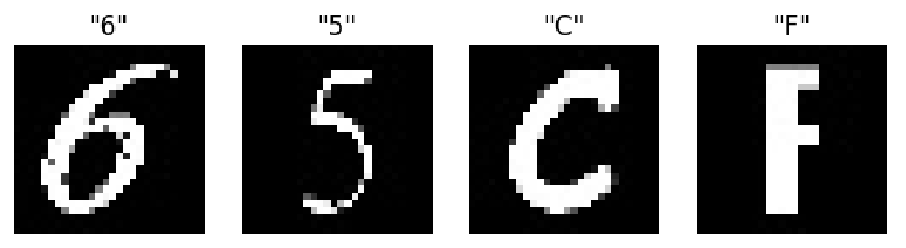
\includegraphics[width=0.9\linewidth]{kennzeichenerkennung/matplotlibbsp.pdf}
    \caption{Beispiel einer Anwendung von Matplotlib}
\end{figure}

Um Matplotlib zu installieren muss das Folgende in der Konsole eingegeben werden:

\begin{listing}[H]
    \begin{minted}{bash}
    pip install matplotlib
    \end{minted}
    \caption{PIP Installation von Matplotlib}
\end{listing}

\paragraph{Keras}\mbox{}\\
Keras ist eine Deep-Learning Schnittstelle für diverse Machine Learning Frameworks wie zum Beispiel Tensorflow oder Theanos. 
Damit wird die Bedienung und Anwendung dieser Frameworks vereinfacht und es bietet auch diverse Funktionen, um Inputs mit 
den Modellen für Maschinelles Lernen kompatibel zu machen. Keras ist ein Teil von Tensorflow, wird aber eigenständig weiterentwickelt, 
um die Kompatibilität mit anderen Machine Learning Frameworks aufrechtzuerhalten. In dieser Applikation wird es in 
Zusammenarbeit mit Tensorflow verwendet, um mit den verwendeten Modellen für Maschinelles Lernen zu arbeiten.\\

Um Keras zu installieren führt man folgenden Befehl in der Konsole aus:

\begin{listing}[H]
    \begin{minted}{bash}
    pip install keras
    \end{minted}
    \caption{PIP Installation von Keras}
\end{listing}

\paragraph{Tensorflow}\mbox{}\\
Tensorflow ist eines der weltweit beliebtesten Frameworks für Maschinelles Lernen und wird von weltweit erfolgreichen Firmen wie 
zum Beispiel Google, AMD oder auch Intel verwendet. Es bietet eine umfassende Plattformen für jegliche Anwendugnen für Maschinelles Lernen 
und ist in Zusammenarbeit mit APIs wie zum Beispiel Keras leicht zu verwenden. In dieser Applikation wird damit ein neuronales 
Netz trainiert und mehrere Modelle für Maschinelles Lernen verwaltet und verwendet.\\

Bei der Installation von Tensorflow muss beachtet werden, dass sich diese von Windows zu Raspbian stark unterscheidet. 
Raspbian unterstützt offiziell die benötigte Version von Tensorflow noch nicht und deswegen muss dieses über ein paar Umwege installiert werden.\\

Windows:\\

Die Installation von Tensorflow unter Windows ist einfach, da man es wie andere Libraries einfach über pip installieren kann.

\begin{listing}[H]
    \begin{minted}{bash}
    pip install tensorflow
    \end{minted}
    \caption{PIP Installation von Tensorflow}
\end{listing}

Raspbian:\\

Bei Raspbian muss Tensorflow manuell kompiliert werden, da die aktuelle Version noch nicht offiziell unterstützt wird. Diese funktioniert 
aber trotz dieses Umweges einwandfrei und wird mit den folgenden Befehlen in der Konsole installiert.\\

Mit dem ersten Befehl werden die benötigten Tools installiert:

\begin{listing}[H]
    \begin{minted}{bash}
    $ sudo apt-get install cmake curl
    \end{minted}
    \caption{Benötigte Tools für Tensorflow}
\end{listing}

Danach kann man die neuste Tensorflow Version von GitHub herunterladen:

\begin{listing}[H]
    \begin{minted}{bash}
    $ wget -O tensorflow.zip https://github.com/tensorflow/tensorflow/archive/v2.4.0.zip
    \end{minted}
    \caption{Tensorflow von GitHub herunterladen}
\end{listing}

Anschließend muss Tensorflow entpackt werden:

\begin{listing}[H]
    \begin{minted}{bash}
    $ unzip tensorflow.zip
    $ mv tensorflow-2.4.0 tensorflow
    $ cd tensorflow
    \end{minted}
    \caption{Entpacken von Tensorflow}
\end{listing}

Im nächsten Schritt müssen noch zusätzlich erforderliche Libraries installiert werden:

\begin{listing}[H]
    \begin{minted}{bash}
    $ ./tensorflow/lite/tools/make/download_dependencies.sh
    \end{minted}
    \caption{Zusätzlich erforderliche Librarys}
\end{listing}

Danach kann die Installation kompiliert werden:

\begin{listing}[H]
    \begin{minted}{bash}
    $ ./tensorflow/lite/tools/make/build_aarch32_lib.sh
    \end{minted}
    \caption{Kompilieren von Tensorflow}
\end{listing}

Danach muss man die Installation mit den folgenden Befehlen abschließen:

\begin{listing}[H]
    \begin{minted}{bash}
    $ cd ~/tensorflow/tensorflow/lite/tools/make/downloads/flatbuffers
    $ mkdir build
    $ cd build
    $ cmake ..
    $ make -j4
    $ sudo make install
    $ sudo ldconfig
    \end{minted}
    \caption{Abschließen der Installation von Tensorflow}
\end{listing}

Nach diesem Schritt sollte Tensorflow Installation funktionieren und man kann es wie jede andere Library in Python einbinden.

\paragraph{local{\_}utils}\mbox{}\\
local{\_}utils ist ein einfaches Python-Script, welches die Arbeit mit WPOD-NET im Bereich der Kennzeichenerkennung vereinfacht 
und in dieser Applikation für die einfachere Nutzung von WPOD-NET verwendet wird. Es beinhaltet die Funktion „detect{\_}lp“ mit 
welcher ein Bild des Kennzeichens und die Koordinaten des Kennzeichens ermittelt werden können. Dieses Script kann über den 
folgenden Link von GitHub heruntergeladen werden: \url{https://github.com/quangnhat185/Plate_detect_and_recognize/blob/master/local_utils.py} 

\paragraph{Scikit-learn}\mbox{}\\
Scikit-learn ist eine freie Library für Maschinelles Lernen und basiert auf Numpy und Matplotlib. Es wird vor allem verwendet, 
um mit großen visuellen Datensätzen neuronale Netze zu trainieren.  Es bietet Funktionen, um Modelle anzupassen, Daten vorzubereiten, 
Modelle zu trainieren und ähnliches. In dieser Applikation wird es für die Normalisierung von Labels verwendet, um diese für Modelle für Maschinelles Lernen anzupassen und für das zufällige Aufteilen von Arrays in Test und Trainingsteile, welche für das Training eines Neuronalen Netzes benötigt werden.\\

Für die Installation von Scikit-learn muss die folgende Zeile in der Konsole ausgeführt werden:

\begin{listing}[H]
    \begin{minted}{bash}
    pip install scikit-learn
    \end{minted}
    \caption{PIP Installation von Scikit-learn}
\end{listing}

\paragraph{Requests}\mbox{}\\
Requests ist eine Library mit welcher HTTP-Anfragen in Python vereinfacht werden. Sie wird häufig verwendet, um mit APIs zu kommunizieren 
und ist eine der beliebtesten Python Librarys, da sie für API-Anwendungen so gut wie notwendig ist. In dieser Applikation wird sie für die 
Kommunikation zu einer eigenen API für den Datenbankzugriff verwendet. Dadurch ist es ohne größere Schwierigkeiten möglich, das Bild des Kennzeichens, 
die ID für den jeweiligen Parkplatz und das Resultat des Kennzeichens an die eigene Datenbank zu senden und auch eine Antwort zu erhalten, ob der 
Zugriff erfolgreich war. Um die Daten mit dieser Library zu übertragen müssen diese einfach nur in einem Dictionary eingetragen werden und dann mit 
dem korrekten Schlüsselwort über die API gesendet werden.\\

Die Installation von Requests erfolgt mit folgendem Befehl in der Konsole:

\begin{listing}[H]
    \begin{minted}{bash}
    pip install requests
    \end{minted}
    \caption{PIP Installation von Requests}
\end{listing}

\paragraph{Gpiozero}\mbox{}\\
Gpiozero ist eine Python-Library für den Raspberry Pi. Mit ihr ist es möglich auf die GPIO-Pins des Raspberry zuzugreifen, Signale von diesen 
auszulesen und Signale an diesen auszugeben. Dies wird oft verwendet, um Sensoren auszuwerten oder um Aktoren zu steuern, da diese Pins frei 
programmierbar sind, wodurch man jede beliebige Anwendung realisieren kann. Der Raspberry Pi kann zwar nur Aktoren in seiner Leistungskategorie ansteuern, 
dies kann aber zum Beispiel mit einem Relais umgangen werden, wodurch der Raspberry Pi zu einem mächtigen Werkzeug für die Sensorik und Aktorik wird. 
Ein Beispiel für die möglichen Anwendungen ist ein Button oder eine Lampe. In dieser Applikation wird mit dieser Library ein gedrückter Button detektiert, 
welcher als Auslöser für die Kamera fungiert.\\

In der folgenden Abbildung sieht man ein Bild der GPIO-Pins des Raspberry Pi, welche mit dieser Library angesteuert werden können:

\begin{figure}[H]
    \centering
    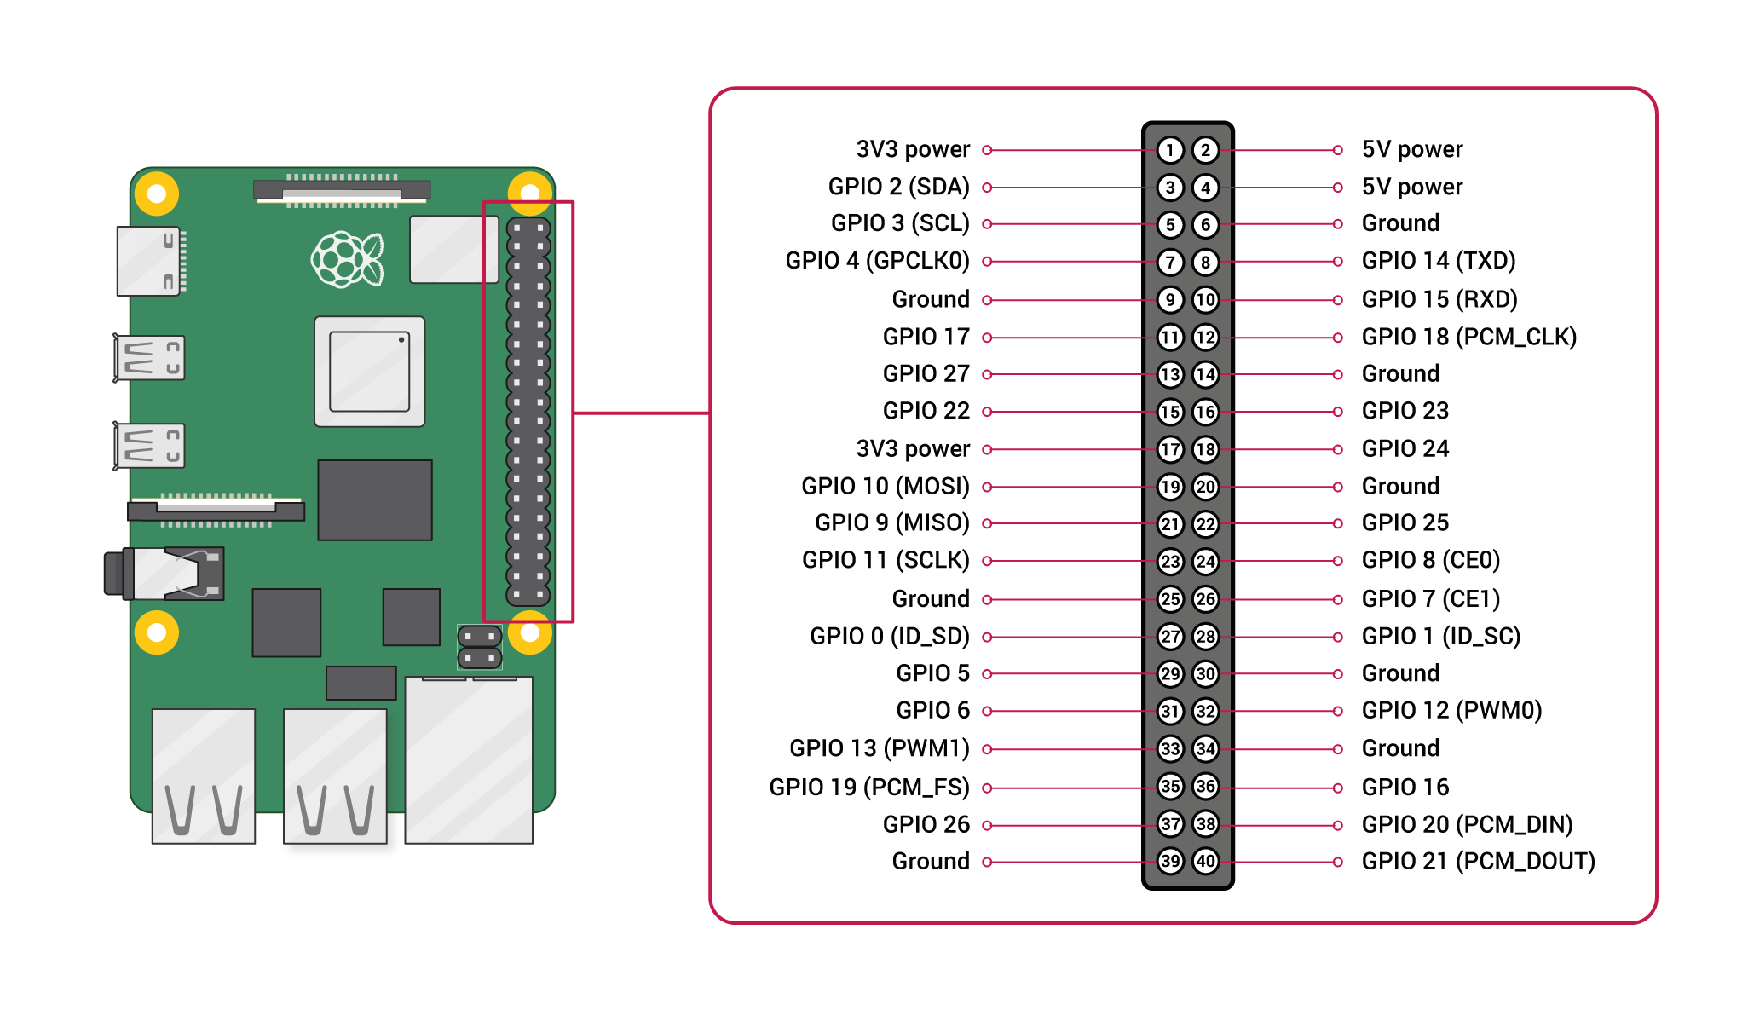
\includegraphics[width=0.8\linewidth]{kennzeichenerkennung/GPIO-Pinout-Diagramm-2.pdf}
    \caption{GPIO-Pins des Raspberry Pi}
\end{figure}

Diese Library kann nur auf dem Raspberry Pi installiert werden. Um die Library Gpiozero zu installieren kann pip verwendet werden:

\begin{listing}[H]
    \begin{minted}{bash}
    pip install gpiozero
    \end{minted}
    \caption{PIP Installation von Gpiozero}
\end{listing}

\paragraph{Picamera}\mbox{}\\
Die Library picamera wird verwendet, um auf das Kameramodul des Raspberry Pi zuzugreifen. Die Library bietet etliche Funktionen an, 
mit welchen die Kamera gesteuert werden kann, wie zum Beispiel Fotos aufzunehmen, Videoaufnahmen zu starten und zu beenden, Fotoeinstellungen 
zu ändern und ähnliches. Die Library ist notwendig, wenn man über Python das Kameramodul bedienen will. In dieser Applikation wird sie verwendet, 
um ein Vorschaubild des aufgenommenen Bildes auf dem Bildschirm darzustellen, falls ein Bildschirm angeschlossen wird und um im 
Anschluss das Bild aufzunehmen und korrekt zu skalieren.\\

Die Installation von picamera ist nur auf dem Raspberry Pi möglich, da nur dieser damit arbeiten kann. 
Für die Installation von picamera muss folgender Befehl in der Konsole eingegeben werden:

\begin{listing}[H]
    \begin{minted}{bash}
    pip install picamera
    \end{minted}
    \caption{PIP Installation von Picamera}
\end{listing}

\subsubsection{Wichtige Programmteile}

Im folgenden Abschnitt werden die wichtigsten Teile des Kennzeichenerkennungsprogrammes genauer betrachtet und erklärt.

\paragraph{WPOD-NET-Modell laden}\mbox{}\\

\begin{listing}[H]
    \begin{minted}{python}
    def load_model(path):
    try:
        path = splitext(path)[0]
        with open ('%s.json' % path, 'r') as json_file:
            model_json = json_file.read()
        model = model_from_json(model_json, custom_objects={})
        model.load_weights('%s.h5' % path)
        print("-> Model loading finished")
        return model
    except Exception as e:
        print(e)
    \end{minted}
    \caption{WPOD-NET Modell laden}
\end{listing}

Für das Lokalisieren des Kennzeichens wird das Model für Maschinelles Lernen WPOD-NET verwendet. Dieses basiert auf YOLOv2, 
mit welchem eine Echtzeitobjekterkennung möglich ist und wurde für diese Anwendung dazu angepasst, dass es möglich ist 
Kennzeichen in einem Bild zu lokalisieren. WPOD-NET versucht zuerst auf Grundlage von YOLOv2 in dem übergebenen Bild 
ein Fahrzeug zu erkennen, erstellt dann auf dieser Grundlage eine Region, in welcher sich mit hoher Wahrscheinlichkeit 
das Kennzeichen befindet und liefert dann die Koordinaten des Kennzeichens im Bild. Im oberen Code sieht man die Funktion 
„load{\_}model“ mit welcher das WPOD-Modell mit den gewichteten Werten geladen wird. Dazu muss dieser Funktion nur der 
Pfad für das WPOD-NET File übergeben werden. Die Funktion versucht dann ein .json-File zu öffnen und erstellt aus 
diesem mit der Funktion „model{\_}from{\_}json“ ein Model mit dem WPOD-NET arbeiten kann. Danach wird im selben Ordner 
in dem auch das .json-File gefunden wurde nach einem .h5-File gesucht. Dieses enthält die gewichteten Werte für das 
Modell und wird dann geladen. Wenn alles funktioniert hat, erhält man als Rückgabe das Modell mit den geladenen Werten. 
Im unteren Code sieht man die Anwendung dieser Funktion. Zuerst wird dabei der Pfad für das WPOD-NET File definiert und 
dieser Pfad wird dann der Funktion „load{\_}model“ übergeben und das Modell als Rückgabewert in der Variable „wpod{\_}net“ abgespeichert.

\begin{listing}[H]
    \begin{minted}{python}
    wpod_net_path = "wpod-net.json"
    wpod_net = load_model(wpod_net_path)
    \end{minted}
    \caption{Anwendung des WPOD-NET Modells}
\end{listing}

\paragraph{Kennzeichen lokalisieren}\mbox{}\\

\begin{listing}[H]
    \begin{minted}{python}
    def get_plate(image_path, Dmax=608, Dmin=256):
        vehicle = preprocess_raw_image(image_path)
        ratio = float(max(vehicle.shape[:2]) / min(vehicle.shape[:2]))
        side = int(ratio * Dmin)
        bound_dim = min(side, Dmax)
        _ , LpImg, _, cor = detect_lp(wpod_net, vehicle, bound_dim, lp_threshold=0.5)
        return LpImg, cor
    \end{minted}
    \caption{get{\_}plate}
\end{listing}

Um das Kennzeichen zu lokalisieren wird die Funktion „get{\_}plate“ angewendet. Dieser Funktion muss man den Pfad für das aufgenommene 
Bild übergeben. Danach wird auf dieses Bild die Funktion „preprocess{\_}raw{\_}image“ angewandt, welches im folgenden Code ersichtlich ist:

\begin{listing}[H]
    \begin{minted}{python}
    def preprocess_raw_image(image_path):
        img = cv2.imread(image_path)
        img = cv2.cvtColor(img, cv2.COLOR_BGR2RGB)
        img = img / 255
        img = cv2.resize(img, (224,224))
        return img
    \end{minted}
    \caption{Bild vorbereiten für WPOD-NET}
\end{listing}

Die Funktion „preprocess{\_}raw{\_}image“ liest das Bild mittels OpenCV ein, ändert dann den Farbraum von BGR zu RGB da OpenCV das Bild mit 
BGR einliest, WPOD-NET aber RGB benötigt und anschließend wird noch die Größe des Bildes angepasst.\\

Danach geht es wieder in der Funktion „get{\_}plate“ weiter. Dort wird danach in den nächsten Codezeilen das Seitenverhältnis des Bildes 
definiert und in einer Variable abgespeichert. Dies ist für die nächste Funktion „detect{\_}lp“ notwendig. Diese Funktion ist eine Hilfsfunktion 
für den Umgang mit WPOD-NET, welcher man das aufgenommene und vorbereitete Bild übergeben muss und als Rückgabe ein Bild des Kennzeichens und 
die Koordinaten des Kennzeichens zurückgibt. Im unteren Codeteil befindet sich die Anwendung der Funktion „get{\_}plate“ wobei bei erfolgreicher 
Anwendung der Funktion noch zusätzlich die Koordinaten des Kennzeichens im Terminal ausgegeben werden.

\begin{listing}[H]
    \begin{minted}{python}
    input_image = image_path[0]
    LpImg,cor = get_plate(input_image)
    print("-> License Plate found in:",splitext(basename(input_image))[0])
    print("-> Coordinates of License Plate: \n", cor)
    \end{minted}
    \caption{Kennzeichen lokalisieren}
\end{listing}

\paragraph{Bild aufnehmen}\mbox{}\\

\begin{longlisting}
    \begin{minted}{python}
    #Kamerabildvorschau
    camera.start_preview(alpha=220)

    #Warten bis Button gedrückt wird
    button.wait_for_press()

    #Altes Bild löschen
    try:
        os.remove('/home/pi/Documents/Kennzeichenerkennung/Plate_examples /image.jpg')
    except OSError:
        pass

    #Bild schießen und abspeichern 
    camera.capture('/home/pi/Documents/Kennzeichenerkennung/Plate_examples /image.jpg')
    camera.stop_preview()
    \end{minted}
    \caption{Bild aufnehmen}
\end{longlisting}

In diesem Codeteil befindet sich die Aufnahme des Fahrzeugbildes. Im ersten Schritt wird dabei die Kameravorschau geöffnet, damit es 
bei einem angeschlossenen Bildschirm einfacher ist das Foto aufzunehmen. Diese Vorschau ist leicht durchsichtig auf dem Bildschirm 
damit man trotzdem alles andere bedienen kann. Danach wird gewartet bis der Button gedrückt wird. Auf diese Weise dient der Button als 
Auslöser für die Kamera. Wenn der Button gedrückt wurde, wird zuerst versucht im gewünschten Zielordner das vorhergehende Bild zu löschen 
damit es zwischen den Bildern zu keinem Konflikt kommt. Dieses vorhergehende Bild wird auch nicht wieder benötigt, da das Bild des 
Kennzeichens im vorhergehenden Programmdurchlauf schon an die Datenbank übergeben wurde. Erst danach wird das eigentliche Foto für 
diesen Programmdurchlauf aufgenommen und im Zielordner abgespeichert. Danach wird die Kameravorschau wieder beendet.

\paragraph{Zeichen mittels Konturerkennung finden}\mbox{}\\

\begin{listing}[H]
    \begin{minted}{python}
    cnt, hierarchy = cv2.findContours(thresh, cv2.RETR_EXTERNAL, cv2.CHAIN_APPROX_SIMPLE)
    \end{minted}
    \caption{Konturen finden}
\end{listing}

Der nächste wichtige Abschnitt des Programmes beschäftigt sich damit, aus dem Kennzeichenbild die einzelnen Zeichen herauszusuchen und einzeln 
darzustellen, damit diese dann von einem weiteren Modell für Maschinelles Lernen erkannt werden können. Dazu wird als erstes die Funktion „findContours“ 
von OpenCV angewendet, welcher man ein binäres Bild des Kennzeichens übergeben muss und als Rückgabe ein Array von Koordinaten aller gefundenen Konturen ausgibt. 

\begin{listing}[H]
    \begin{minted}{python}
    def sort_contours(contours):
        i = 0
        boundingBoxes = [cv2.boundingRect(c) for c in contours]
        (contours, boundingBoxes) = zip(*sorted(zip(contours, boundingBoxes), key=lambda b: b[1][i], reverse = False))
        return contours
    \end{minted}
    \caption{Konturen sortieren}
\end{listing}

Im nächsten Schritt wird die Funktion „sort{\_}contours“ benötigt, welche die Konturen aus dem vorherigen Array sortiert. Sortieren bedeutet dabei, 
dass zuerst Rechtecke bei den Konturen aufgespannt werden und mit diesen die Konturen von links nach rechts geordnet werden, damit sich am Ende beim Resultat 
des Kennzeichens die korrekte Reihenfolge ergibt.

\begin{listing}[H]
    \begin{minted}{python}
    for c in sort_contours(cnt):
        (x, y, w, h) = cv2.boundingRect(c)
        if h / lp_img.shape[0] >= 0.5 and h / lp_img.shape[0] <= 0.95: 
            seperated = erosion[y:y+h,x:x+w]
            seperated = cv2.resize(seperated, dsize=(30, 60))
            hierarchy, seperated = cv2.threshold(seperated, 220, 255, cv2.THRESH_BINARY + cv2.THRESH_OTSU)
            found_characters.append(seperated)

    print("-> Detected {} characters".format(len(found_characters)))
    \end{minted}
    \caption{Filterung der korrekten Konturen}
\end{listing}

\paragraph{Bildverarbeitung}\mbox{}\\

Im gesamten Programm wird ab und zu ein Bildverarbeitungsalgorithmus verwendet, aber zwischen der Kennzeichenlokalisierung und der Zeichenerfassung befindet 
sich der Hauptteil davon. Um die einzelnen Zeichen zu lokalisieren müssen zuvor einige Bildverarbeitungsalgorithmen und Funktionen angewandt werden und 
an anderen Stellen werden meistens die gleichen Funktionen angewandt wie dort. Im folgenden Code sieht man diese Bildverarbeitung:

\begin{listing}[H]
    \begin{minted}{python}
    lp_img = cv2.convertScaleAbs(LpImg[0], alpha=(255))
    api_img = cv2.cvtColor(lp_img, cv2.COLOR_BGR2RGB)
    gray = cv2.cvtColor(lp_img, cv2.COLOR_BGR2GRAY)
    blur = cv2.bilateralFilter(gray, 11, 15, 15)
    thresh = cv2.threshold(blur, 127, 255, cv2.THRESH_BINARY_INV + cv2.THRESH_OTSU)[1]
    kernel = cv2.getStructuringElement(cv2.MORPH_RECT, (3, 3))
    erosion = cv2.erode(thresh, kernel, iterations=1)
    \end{minted}
    \caption{Bildverarbeitungsalgorithmen}
\end{listing}

In der ersten Zeile wird auf das Kennzeichenbild die Funktion „convertScaleAbs“ angewandt welche jeden Array-Eintrag zu einem Farbwert konvertiert mit dem 
OpenCV arbeiten kann. Danach wird in einem eigenen Schritt der Farbraum von BGR zu RGB gewechselt, da die API für die Übertragung zur Datenbank ein RGB-Bild 
des Kennzeichens benötigt. Für die eigentliche Weiterverarbeitung wird der Farbraum in der nächsten Zeile von BGR zu einem Graustufenbild geändert. 
Anschließend wird darauf ein bilaterales Filter angewandt, welches unnötiges Bildrauschen entfernt, um die weiteren Schritte zu vereinfachen. Danach 
wird auf das dadurch entstandene Bild Thresholding angewandt, um es in ein binäres Bild zu konvertieren, welches für die Konturerkennung notwendig ist. 
Um die Qualität dieses binären Bildes noch etwas zu verbessern wird danach mit einem 3x3 Kernel Erosion verwendet. Danach ist das Bild fertig vorbereitet für die Konturerkennung.

\paragraph{Visualisierung mittels Matplotlib}\mbox{}\\

Um die einzelnen Bildverarbeitungsmechanismen zu überprüfen, die Werte anzupassen oder relevante Daten darzustellen, ist es hilfreich mit Hilfe der Library 
Matplotlib eine Visualisierung durchzuführen. Zusätzlich wird auch noch Jupyter Notebook verwendet, wodurch die Visualisierung nur in der Web-Applikation 
sichtbar ist, und damit werden nicht unzählige Tabs geöffnet. Im unteren Code sieht man eine solche Anwendung von Matplotlib.

\begin{listing}[H]
    \begin{minted}{python}
    mplt.figure(figsize=(10,5))
    mplt.subplot(2,2,1)
    mplt.axis(False)
    mplt.imshow(gray, cmap='gray', vmin = 0, vmax = 255) 
    mplt.subplot(2,2,2)
    mplt.axis(False)
    mplt.imshow(blur, cmap='gray', vmin = 0, vmax = 255)
    mplt.subplot(2,2,3)
    mplt.axis(False)
    mplt.imshow(thresh, cmap='gray', vmin = 0, vmax = 255)
    mplt.subplot(2,2,4)
    mplt.axis(False)
    mplt.imshow(erosion, cmap='gray', vmin = 0, vmax = 255)
    \end{minted}
    \caption{Anwendung einer Visualisierung mit Matplotlib}
\end{listing}

Prinzipiell funktioniert die Library Matplotlib gleich wie eine figure in MATLAB. Im oberen Codeteil werden damit die einzelnen Bildverarbeitungsalgorithmen 
dargestellt. Zuerst muss eine figure erstellt werden, in welcher die einzelnen Subplots platziert werden. Damit kann man die zusammengehörenden Visualisierungen 
gruppieren. Danach muss für jedes Bild ein eigener Subplot erzeugt werden, welchen man mit den mitgegebenen Parametern in der figure platzieren kann. Danach 
wird bei allen Bildern die Achsenbeschriftung deaktiviert, da diese hier nicht benötigt wird. Danach wird das gewünschte Bild ausgewählt und da alle Bilder in 
Graustufen sind, wird diese angepasst und der Farbwertebereich auf 0 bis 255 gesetzt. Im unteren Bild sieht man die Ausgabe dieser Visualisierung.

\begin{figure}[H]
    \centering
    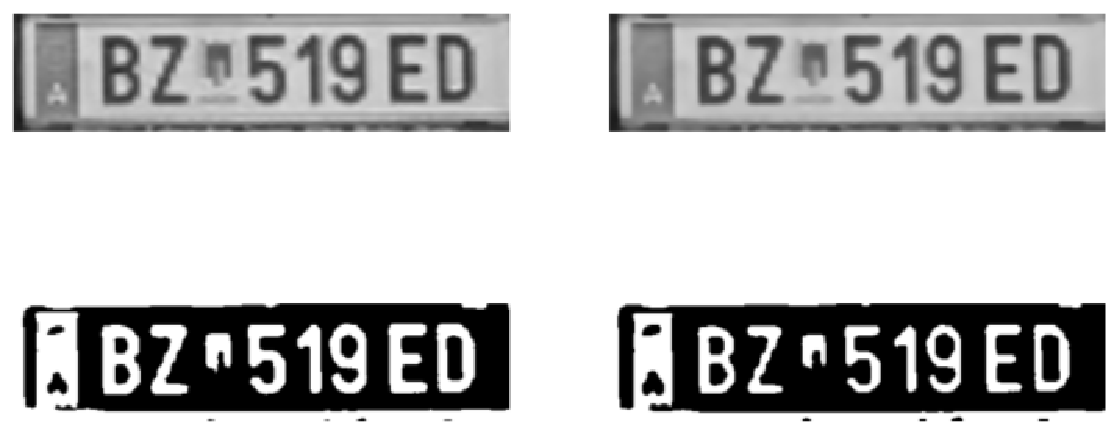
\includegraphics[width=0.9\linewidth]{kennzeichenerkennung/matplotlibvisual.pdf}
    \caption{Visualisierung mit Matplotlib}
\end{figure}

\paragraph{Modell für Zeichenerkennung laden und anwenden}\mbox{}\\

Für die Zeichenerkennung wird ein eigenes Neuronales Netz verwendet, welches auf MobileNetV2 basiert. Dafür wird primär die Funktion „predict{\_}from{\_}model“ 
verwendet, welche im unteren Code ersichtlich ist.

\begin{listing}[H]
    \begin{minted}{python}
    def predict_from_model(image, model, labels):
        image = cv2.resize(image,(80, 80))
        image = npy.stack((image,)*3, axis = -1)
        prediction = labels.inverse_transform([npy.argmax (model.predict(image[npy.newaxis,:]))])
        return prediction
    \end{minted}
    \caption{predict{\_}from{\_}model}
\end{listing}

Vor der Anwendung dieser Funktion muss wieder, wie beim ersten Modell für Maschinelles Lernen, das Modell zuerst geladen werden. Danach kann diese Funktion verwendet werden, 
welcher man das Bild einer Zeichens und das Model übergeben muss. Die Funktion „predict{\_}from{\_}model“ wendet dann nur dieses Modell an und übergibt das 
vermutete Ergebnis in ein Array.

\begin{longlisting}
    \begin{minted}{python}
    fig = mplt.figure(figsize = (15,3))
    cols = len(found_characters)
    grid = gridspec.GridSpec(ncols= cols, nrows= 1, figure = fig)

    result = ''
    for i, character in enumerate(found_characters):
        fig.add_subplot(grid[i])
        title = npy.array2string(predict_from_model(character, model, labels))
        mplt.title('{}'.format(title.strip("'[]"), fontsize=20))
        result += title.strip("'[]")
        mplt.axis(False)
        mplt.imshow(character, cmap='gray')

    print("-> License Plate:", result)
    \end{minted}
    \caption{Anwendung der Zeichenerkennung}
\end{longlisting}

Im oberen Bild sieht man die Anwendung der vorherigen Funktion. Prinzipiell wird für jedes vorher gefundene Zeichen das Modell angewendet 
und das Resultat von einem Array zu einem String konvertiert. Dieser String wird dann zum Ergebnis-String hinzugefügt, wodurch man am Ende das 
komplette Kennzeichen in einem String hat. Zusätzlich wird das komplette Kennzeichen mit den vermuteten Ergebnissen mit Matplotlib visualisiert. 
Dies ist im unteren Bild ersichtlich.

\begin{figure}[H]
    \centering
    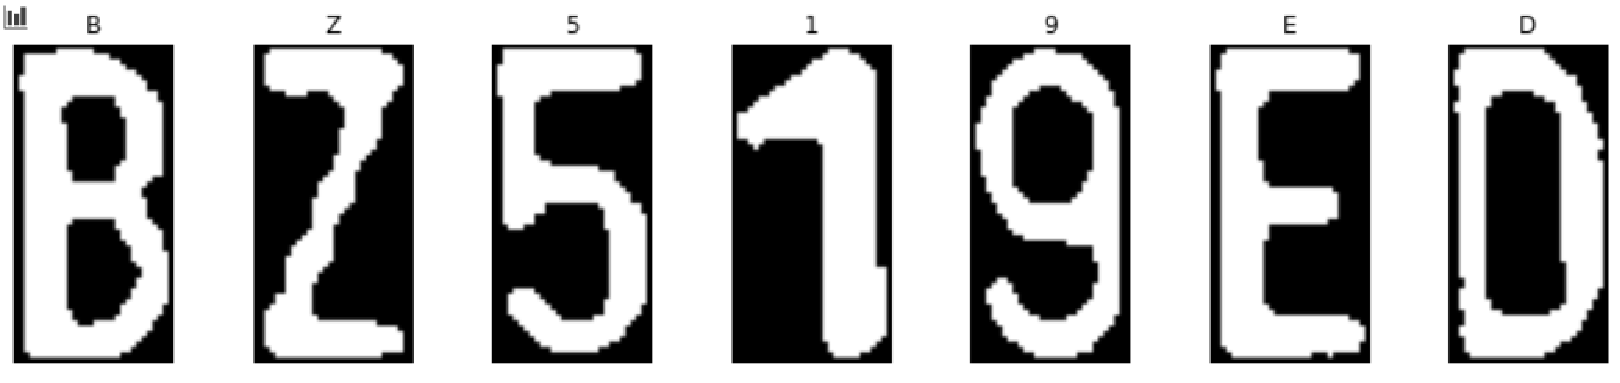
\includegraphics[width=0.9\linewidth]{kennzeichenerkennung/Ergebnisvisual.pdf}
    \caption{Visualisiertes Ergebnis der Kennzeichenerkennung}
\end{figure}

\paragraph{Resultat mittels API an Datenbank senden}\mbox{}\\

Wenn das Programm zu einem Resultat gekommen ist, muss dieses noch an die Datenbank übergeben werden. Der dafür zuständige Code ist im nächsten Codeteil ersichtlich.

\begin{longlisting}
    \begin{minted}{python}
    #API-Definitionen
    url = "http://dev.philipp-kraft.com/api/v1/detections"
    lp_result = {}
    lp_files = {}
    lp_result["name"] = result 
    lp_result["parking_lot_id"] = "2"   #Parkplatz-ID 
    lp_files=[
    ('image',('kennzeichen.png',open('lp_image/lp.png','rb'),'image/png'))
    ]
    header = {"Authorization": "Bearer 5|4NcJgCrR9FkeTFeTvRGHLQqoJBeY8IDqxborpuuS"}

    #Senden der Daten an die Datenbank und Ausgabe der Response
    resp = requests.post(url, data=lp_result, files=lp_files, headers=header)
    print("-> API-Response:",resp.text)
    \end{minted}
    \caption{Senden der Ergebnisse an die Datenbank}
\end{longlisting}

Im ersten Schritt werden die URL für die API und für die Ergebnisse zwei Dictionaries erstellt. In das erste Dictionary wird der String für das Kennzeichen 
und die ID-Nummer des Parkplatzes eingetragen. In das zweite Dictionary kommt das Bild des Kennzeichens. Im nächsten Schritt muss noch ein Bearer Token 
definiert werden, welcher auf der APM-Website generiert werden kann. Dieser wird zur Autorisierung benötigt. Danach können diese Daten über einen Post-Befehl 
an die API gesendet werden. Um den Status dieser Kommunikation zu überprüfen wird im Anschluss noch die Antwort der API im Terminal ausgegeben. Bei 
erfolgreicher Kommunikation antwortet diese mit dem aktuellen Status des Fahrzeuges auf dem Parkplatz.

\subsection{Raspberry Pi}

\subsubsection{Einleitung}
Damit die Software der Kennzeichenerkennung arbeiten kann, benötigt es eine geeignete Hardware. Diese muss dabei die folgenden Eigenschaften 
aufweisen, um für die Kennzeichenerkennung geeignet zu sein:

\begin{itemize}
    \item Möglichst klein
    \item Nicht zu teuer 
    \item Möglichkeit eine Kamera anzuschließen 
    \item Schnell 
    \item Internetanbindung
\end{itemize}

\subsubsection{Wahl des Raspberry Pi}
In dieser Applikation wird ein RaspberryPi 4B 2GB verwendet, da er alle zuvor genannten Eigenschaften am besten erfüllt.\\

\begin{figure}[H]
    \centering
    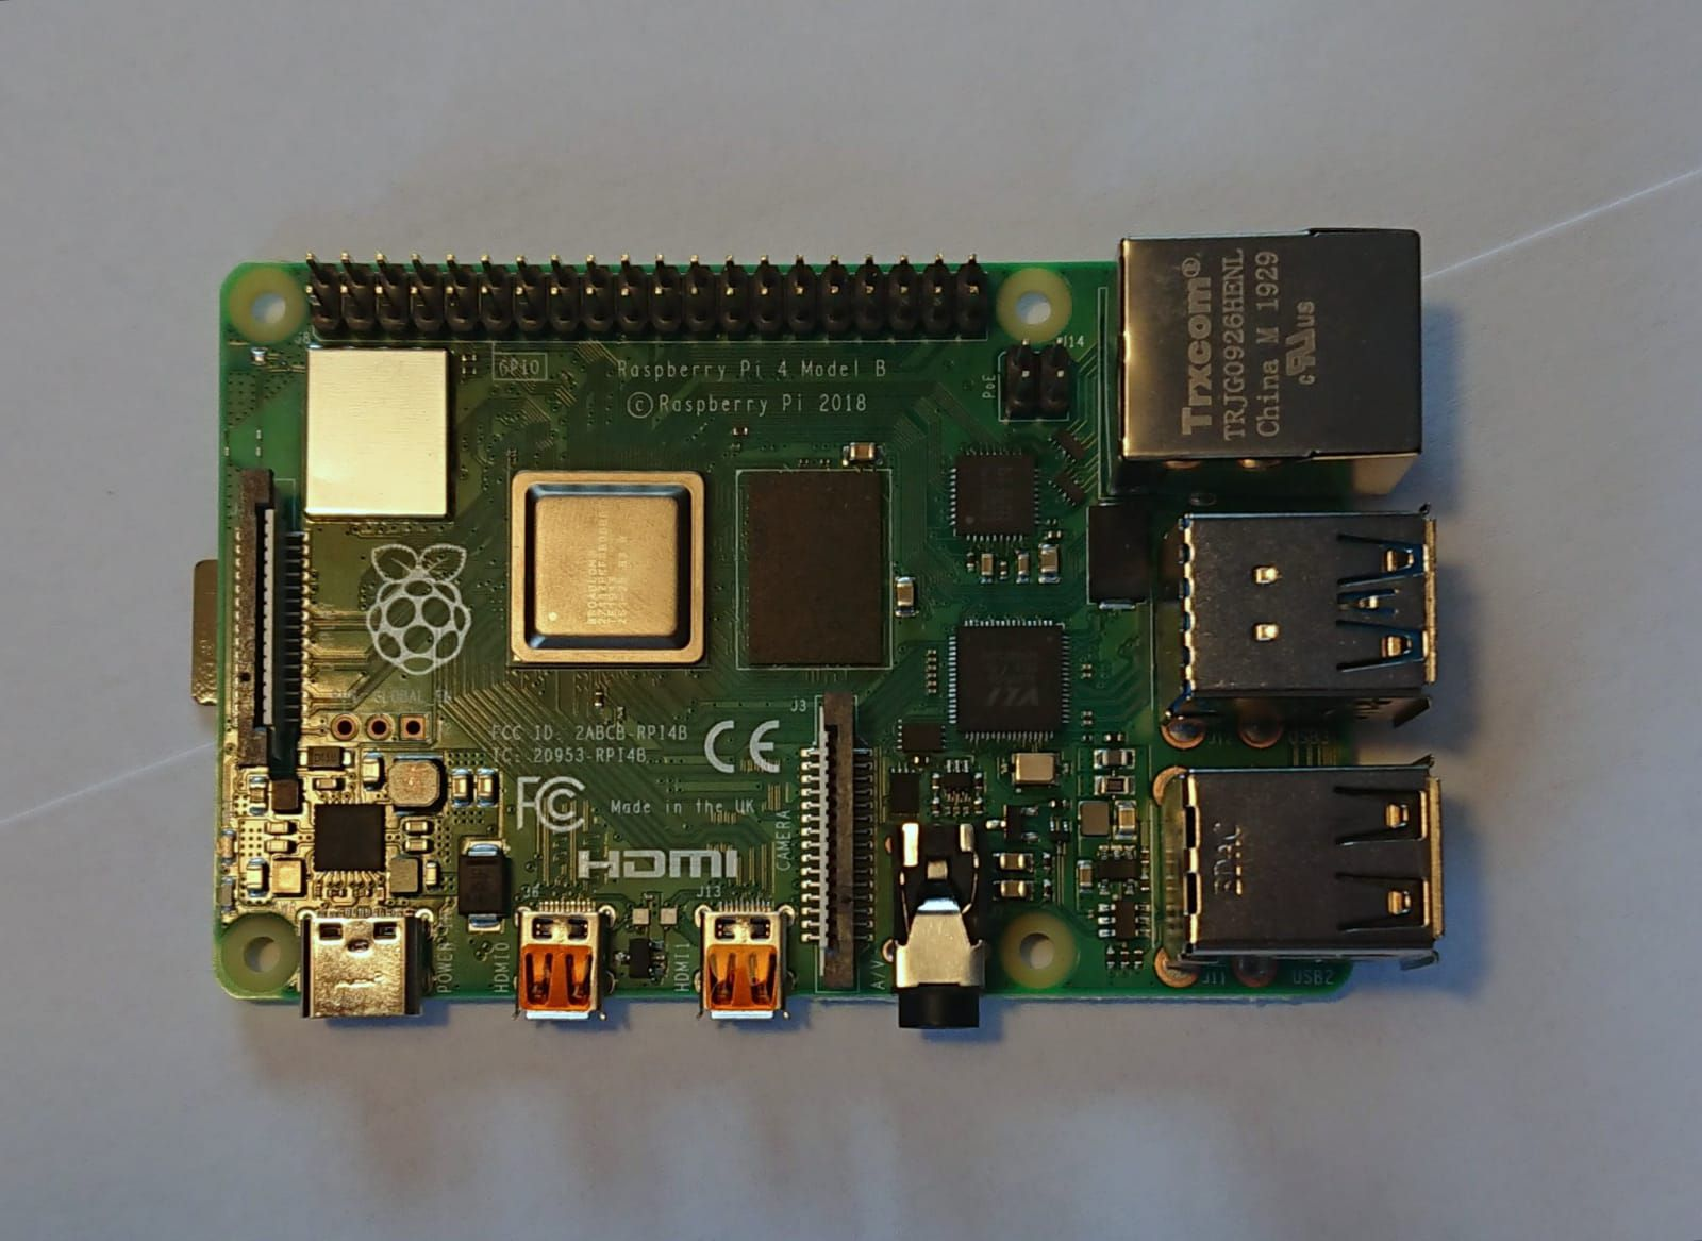
\includegraphics[width=0.6\linewidth]{kennzeichenerkennung/rpi.pdf}
    \caption{Raspberry Pi}
\end{figure}

Er hat die Größe einer Scheckkarte, wodurch es möglich ist ein kompaktes Gehäuse zu bauen, welches man einfach montieren kann. 
Er ist mit 35€ pro Stück nicht zu teuer. Er hat einen integrierten Kameraanschluss und es gibt unzählige Kameras, welche damit 
kompatibel sind. Er hat für seine Größe eine sehr gute Rechenkraft und ist damit in der Lage das komplette Programm für die 
Kennzeichenerkennung in einer akzeptablen Zeit abzuarbeiten. Er besitzt außerdem einen Ethernet-Anschluss und ein WLAN-Modul, 
wodurch er sehr einfach mit dem Internet verbunden werden kann.

\subsubsection{Kamera}
Für den Raspberry Pi muss zudem noch die passende Kamera ausgewählt werden, um die Bilder von den Kennzeichen aufzunehmen. 
Dafür gibt es Unmengen an kompatiblen Kameras, aber hier wird das Originalzubehör von RaspberryPi verwendet. Dies hat den Grund, 
dass diese Kamera leicht zu verwenden, sehr klein, mit Schrauben einfach zu befestigen und günstig ist. Zudem liefert sie ein 
qualitativ hochwertiges Bild, welches für die Software gut verarbeitbar ist.

\begin{figure}[H]
    \centering
    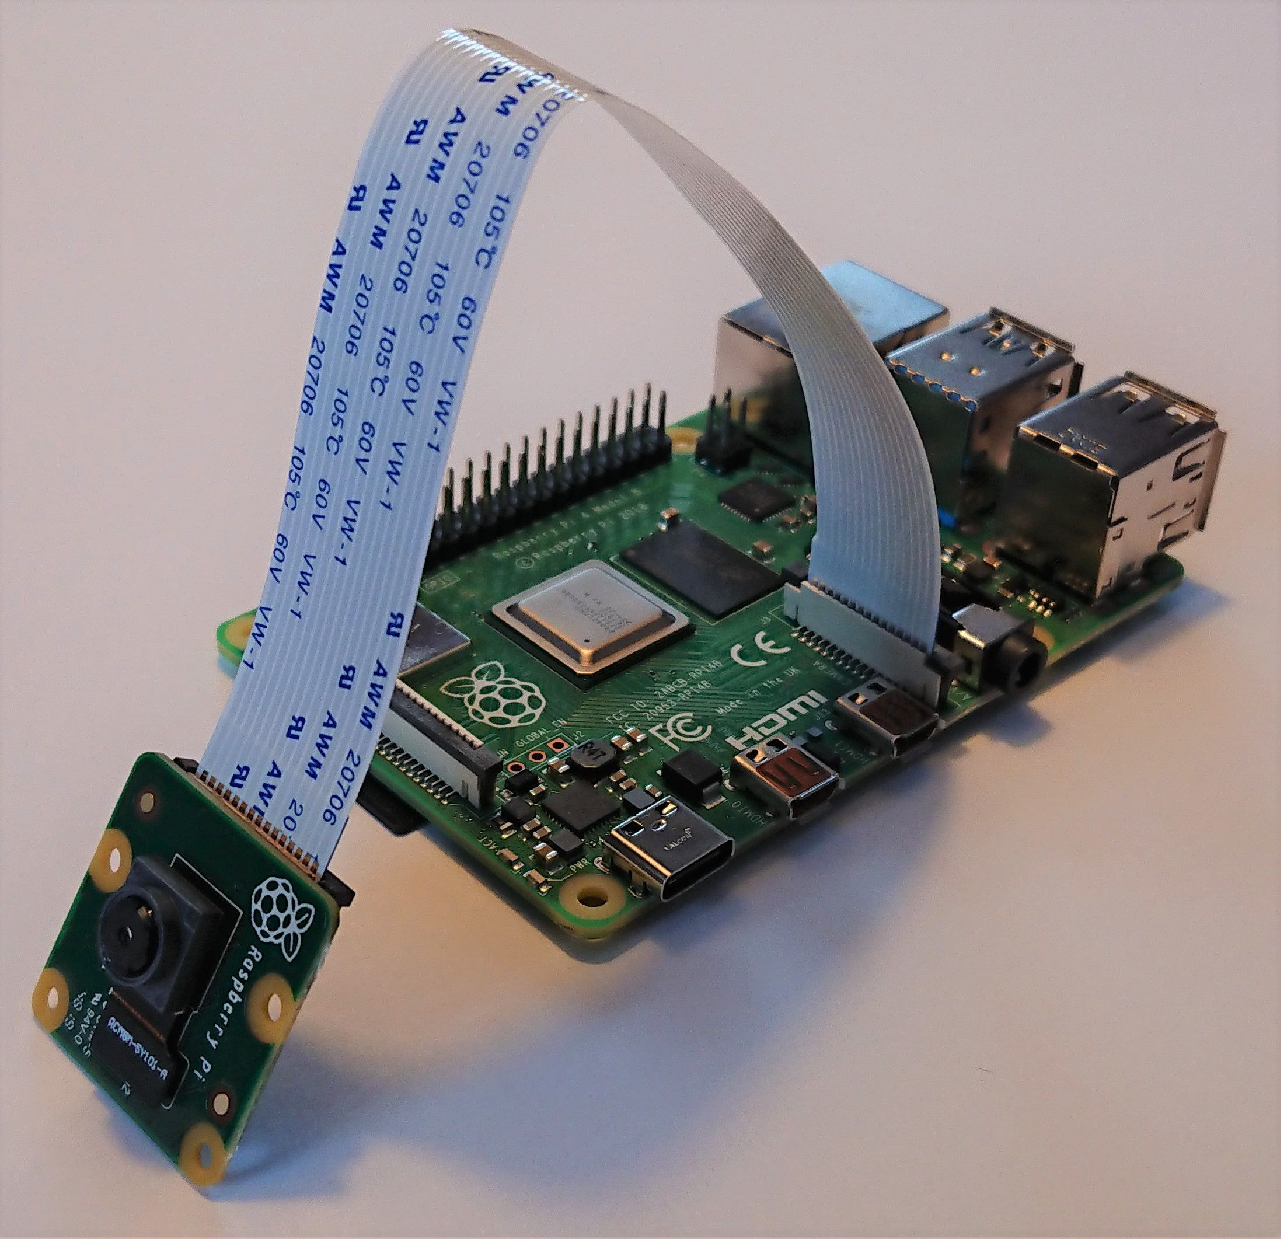
\includegraphics[width=0.6\linewidth]{kennzeichenerkennung/rpiKamera.pdf}
    \caption{Raspberry Pi mit Kamera}
\end{figure}

\subsection{Maschinelles Lernen}

\subsubsection{Einleitung}
Die Kennzeichenerkennung ist eine sehr komplexe Anwendung, da es unzählige Kennzeichen gibt und jedes einzelne davon erkannt werden sollte. 
Dabei ist nicht nur auf verschiedene Länderkennzeichen zu achten, welche sich stark voneinander unterscheiden, sondern auch auf Sonderkennzeichen, 
welche sich sogar auf nationaler Ebene von den normalen Kennzeichen unterscheiden. Zudem besteht noch die Problematik, dass sich die Kennzeichen 
oft in unterschiedlichen Zuständen befinden, wie zum Beispiel mit Dreck beschmutzt oder ähnliches. Das bedeutet, dass eine in der Praxis 
anwendbare Kennzeichenerkennung mit all diesen Gegebenheiten zurechtkommen muss, damit das Kennzeichen in nahezu jeder möglichen Situation 
erkannt werden kann. Um dies zu erreichen wird das Programm für die Kennzeichenerkennung in drei größere Teile aufgeteilt. Die Kennzeichenlokalisierung, 
die Zeichenerfassung und die Zeichenerkennung. Die Zeichenerfassung gestaltet sich relativ einfach, da diese bereits ein Bild des Kennzeichens erhält, 
in dem ansonsten keine größeren Störfaktoren beinhaltet sind. Diese muss also nur die Konturen innerhalb dieses Bildes finden und diese so sortieren, 
dass nur noch die einzelnen Zeichen übrig bleiben. Bei der Kennzeichenlokalisierung und der Zeichenerfassung gestaltet sich die Lage schon etwas schwieriger. 
Die Kennzeichenlokalisierung steht vor dem Problem, dass wenn man klassisch mit der Bildverarbeitung nach einer passenden Kontur für das Kennzeichen sucht, 
kann dieser Algorithmus durch Störfaktoren wie ein zufällig ähnlich großes Orts- oder Straßenschild getäuscht werden, wodurch es zu einem Fehler kommt. 
Auch Fenster oder ähnlich proportionierte Gegenstände können zu solch einem Fehler führen. Die Lösung dafür befindet sich im Bereich des Maschinellen Lernens. 
Anstatt nur nach einer Kontur zu suchen, wird mit solch einem Modell gezielt nach einem Kennzeichen gesucht. Dies ist möglich, da so ein Modell mit vielen 
möglichen Eingaben und den passenden Ausgaben dazu trainiert wird ein Muster zwischen den Ein- und Ausgaben zu finden, mit welchem es dann ähnliche Probleme 
selbstständig lösen kann. Auch bei der Zeichenerkennung bietet sich solch ein Modell an, da es darauf trainiert werden kann, einzelne Zeichen mit einer 
hohen Genauigkeit zu erkennen. Hier wäre es zwar ohne Maschinelles Lernen auch möglich ein relativ gutes Ergebnis zu erzielen, indem man mittels Korrelation 
von Vergleichsbildern das Zeichen findet, welches am wahrscheinlichsten passen würde, aber in dieser Applikation wird auch hierfür ein Modell für Maschinelles Lernen verwendet.

\subsubsection{Definition}
Maschinelles Lernen beschreibt ein Modell, welches zuerst in einer Trainingsphase trainiert werden muss, um danach ähnliche Probleme näherungsweise lösen zu können. 
Dazu wird in der Trainingsphase ein Datensatz bereitgestellt welcher mögliche Eingaben und meistens auch die passenden Ausgaben enthält. Durch die vielen verschiedenen 
Eingaben und Ausgaben ist es für das Modell möglich ein Muster zwischen diesen zu erkennen, welches durch dieses Training verbessert werden kann. Es gilt dabei, je 
länger die Trainingsphase dauert desto genauer wird das Modell. Der Aufwand besteht dabei darin, die gigantischen Datensätze zur Verfügung zu stellen, da diese oft 
zuvor erstellt werden müssen. Zudem ist das Training ein sehr rechenintensiver Vorgang, welcher für ein gutes Ergebnis oft mehrere Stunden benötigt. In den letzten 
Jahren hat sich im Bereich des Modell Trainings eine neue Entwicklung namens „Deep Learning“ verbreitet, mit welcher eine höhere Genauigkeit als mit bisherigen Modellen 
erreicht werden kann. Dabei werden künstliche Neuronale Netze erstellt, welche der Vernetzung von Neuronen in Lebewesen nachempfunden sind. Diese künstlichen Neuronen 
sind Verknüpfungspunkte zwischen Eingang und Ausgang des Modells und sind je nach Komplexität in verschiedene Schichten aufgeteilt. Um diese künstlichen Neuronen zu 
trainieren, werden deren Gewichtungswerte angepasst. Deswegen muss bei solchen Modellen auch oft eine Datei mit den gewichteten Werten eingebunden werden.

\subsubsection{Vergleich Maschinelles Lernen / Bildverarbeitung}
Zum Beginn dieser Applikation wurde ein Ansatz ohne den Einsatz von Maschinellem Lernen verfolgt. Dazu wurde ein Testprogramm geschrieben, welches das Kennzeichen 
über eine Konturerkennung lokalisieren sollte. Dies führte aber zu häufig auftretenden Fehlern. Einer dieser Fehler ist in der unteren Abbildung ersichtlich.

\begin{figure}[H]
    \centering
    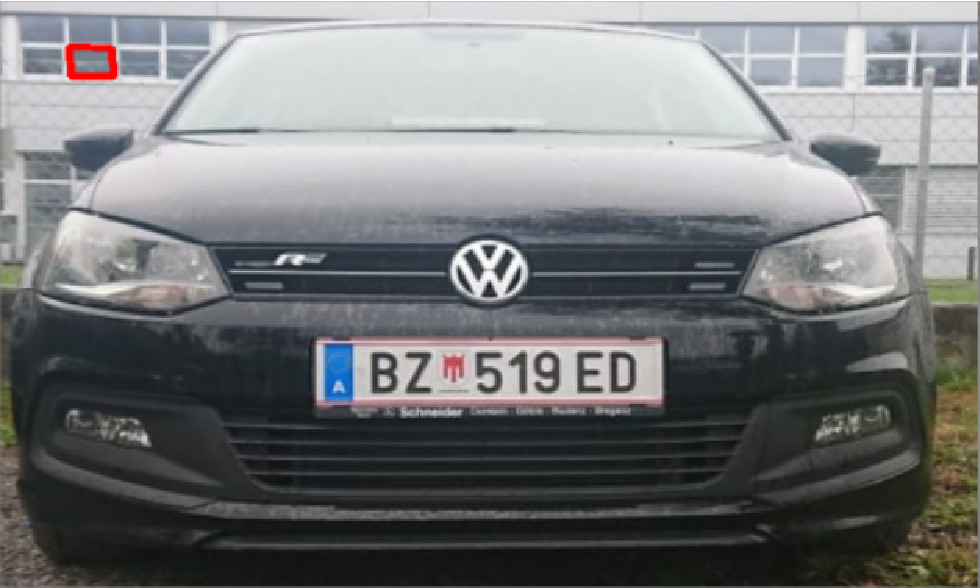
\includegraphics[width=0.9\linewidth]{kennzeichenerkennung/bildvtestfehler.pdf}
    \caption{Fehler bei Konturerkennung}
\end{figure}

Wie in der oberen Abbildung erkennbar ist, hat das Programm nicht das Kennzeichen erkannt, sondern ein Fenster im Hintergrund, welches eine ähnliche Kontur 
wie das Fenster aufweist. Dies ist deswegen aufgetreten, da das Kennzeichen über seine Kontur gefunden werden sollte und dazu alle Konturen im Bild aufgelistet 
werden und aus dieser Liste dann das Kennzeichen herausgesucht werden sollte. Dies führte in dieser Testversion aber nahezu nie zu einem Ergebnis, welches in 
der Praxis anwendbar gewesen wäre. Durch eine Anpassung der Software wäre es zwar möglich gewesen die Genauigkeit zu verbessern und dafür zu sorgen, dass mit 
einer größeren Wahrscheinlichkeit die richtige Kontur ausgewählt wird, aber bei einer Kontur mit den gleichen Proportionen wie ein Kennzeichen, wäre die Konturerkennung 
wieder schnell an ihre Grenzen gestoßen. Deswegen wurde der Ansatz komplett verändert und für die Kennzeichenlokalisierung ein Modell für Maschinelles Lernen 
verwendet, welches auf deutlich elegantere und effizientere Weise ein besseres Resultat erzielen kann.

\begin{figure}[H]
    \centering
    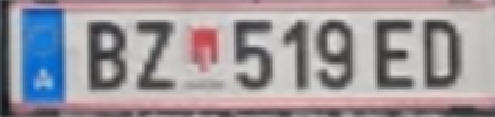
\includegraphics[width=0.5\linewidth]{kennzeichenerkennung/kennmaschinlearn.pdf}
    \caption{Resultat mit maschinellem Lernen}
\end{figure}

Zum Vergleich mit dem Testprogramm sieht man im oberen Bild das Ergebnis der Variante mit Maschinellem Lernen mit demselben Eingangsbild. Dabei wurde ohne 
Probleme das Kennzeichen perfekt erkannt und im weiteren Programmablauf aus dem Eingangsbild ausgeschnitten.

\subsubsection{Verwendete Modelle für Maschinelles Lernen}

\paragraph{WPOD-NET}\mbox{}\\
Das „Warped Planar Object Detection Network“ (WPOD-NET) ist ein künstliches Neuronales Netz, welches von Sérgio Montazolli Silva und 
Cláudio Rosita Jung\footnote{Montazzolli, Sérgio \& Jung, Claudio. (2018). License Plate Detection and Recognition in Unconstrained Scenarios. } 
entwickelt wurde. Es wurde entwickelt, um aus Bildern die Kennzeichen von Fahrzeugen herauszusuchen und bietet im Gegensatz zu anderen Modellen den entscheidenden 
Vorteil, dass es bei diesem Modell irrelevant ist aus welchem Winkel das Bild vom Kennzeichen aufgenommen wird. Andere Modelle funktionieren oft nur wenn das Foto 
vom Kennzeichen direkt von vorne aufgenommen wurde, da ansonsten das Bild verzerrt wird und dadurch das Kennzeichen nicht mehr ausgelesen werden kann. Dieses Modell 
schafft es auch aus einem von der Seite aufgenommen Bild das Kennzeichen in den meisten Fällen gut genug herauszulesen, dass dieses Bild danach weiterverarbeitet 
werden kann. Dies bietet den Vorteil, dass die Kamera für das Gerät nicht in fix verbaut werden muss, sondern theoretisch auch in einem mobilen Gerät installiert werden kann.\\

Die Kennzeichenerkennung dieses Modells basiert auf zwei Schritten. Zuerst wird im Bild nach einem Fahrzeug gesucht und dieses ausgeschnitten, um danach mit 
WPOD-NET das Kennzeichen aus diesem Bild herauszusuchen. Die Fahrzeugerkennung basiert dabei auf dem 
YOLOv2\footnote{J. Redmon and A. Farhadi, "YOLO9000: Better, Faster, Stronger," 2017 IEEE Conference on Computer Vision and Pattern Recognition (CVPR), Honolulu, HI, USA, 2017, pp. 6517-6525, doi: 10.1109/CVPR.2017.690.} Netzwerk, 
welches für Echtzeitobjekterkennung verwendet wird und neben vielen anderen Gegenständen auch in der Lage ist Fahrzeuge zu erkennen. Nach dieser Fahrzeugerkennung wird das Bild in das WPOD-NET eingegeben.

\begin{figure}[H]
    \centering
    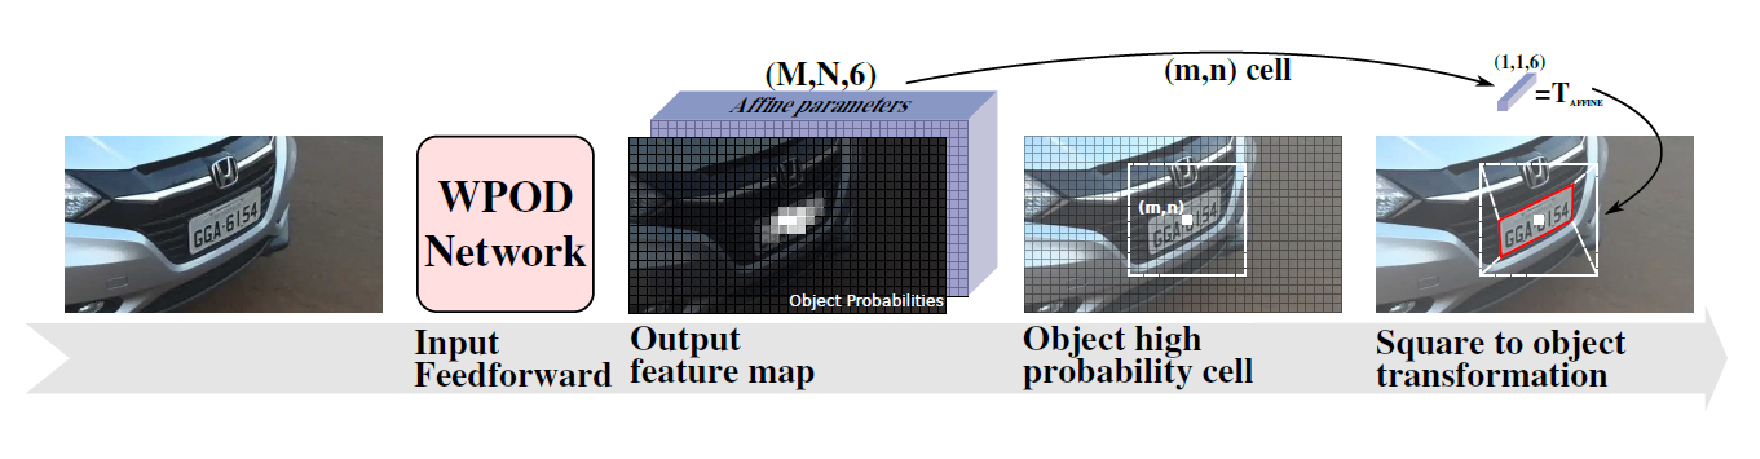
\includegraphics[width=0.9\linewidth]{kennzeichenerkennung/wpodnet.pdf}
    \caption{Ablauf von WPOD-NET}
\end{figure}

Im oberen Bild ist der prinzipielle Ablauf der Kennzeichenerkennung ersichtlich. Zu Beginn wird das Bild mit dem Kennzeichen in das WPOD-NET eingegeben 
und dieses gibt dann eine Matrix mit gewichteten Werten zurück, welche für jede einzelne Zelle eine Wahrscheinlichkeit angibt, dass sich dort ein Kennzeichen 
befindet. Um die Zelle, die am wahrscheinlichsten ist, wird dann ein Rechteck gespannt in welchem sich mit sehr hoher Wahrscheinlichkeit das Kennzeichen 
befindet. Danach wird auf die Wahrscheinlichkeitswerte für das gesamte Rechteck Thresholding angewandt, um zu bestimmen in welchen Zellen sich das Kennzeichen 
befindet. Dadurch hat man dann diejenige Region gefunden, in der sich das Kennzeichen befindet und kann dieses, wenn nötig in ein horizontal und vertikal 
ausgerichtet Rechteck umwandeln. Dadurch erhält man dann ein Bild des Kennzeichens.

\paragraph{MobileNetV2}\mbox{}\\
MobileNetV2 ist die Grundlage für das eigene trainierte Neuronale Netz. MobileNetV2 ist eine Grundlage für diverse Neuronale Netze und speziell für Anwendungen im Bereich der Computer Vision 
geeignet. Einige Beispiel dafür sind die Erkennung von Gesichtsmerkmalen, Echtzeitobjekterkennung, Unterscheidung diverser Hunderassen oder ähnliches. Dabei ist das Modell je nach Bedürfnissen 
einstellbar, womit für eine schnellere und bessere Leistung weniger Schichten für das Neuronale Netz verwendet werden, oder aber für eine sehr genaue und präzise Funktion mehr Schichten verwendet werden. 
Dies ist dadurch möglich, dass das Netzwerk auf einer variablen Schichtanzahl aufgebaut ist. In dieser Applikation wird es deswegen verwendet, da damit in diesem Bereich eine hohe Präzision erzielbar ist, 
welche für die Kennzeichenerkennung benötigt wird.

\subsection{Modell Training}
Um das Modell für die Zeichenerkennung zu trainieren wurde ein eigenes Programm geschrieben, welches das Modell mittels Tensorflow trainiert. 
Dazu wird ein Datensatz von 35 000 Bildern von Zeichen verwendet, bei welchen die richtige Ausgabe aus dem Dateiname auslesbar ist. 
Im folgenden Bild sieht man ein Beispiel für so ein Bild aus dem Datensatz.

\begin{figure}[H]
    \centering
    
\includegraphics[width=0.2\linewidth]{kennzeichenerkennung/S.pdf}
    \caption{Beispiel eines Zeichens aus dem Datensatz}
\end{figure}

Das Modell wird durch die verschiedenen Schriftarten und die variierende Qualität der Bilder nicht direkt auf die Erkennung von Zeichen aus 
einem Kennzeichen trainiert, sondern auf die Erkennung von Zeichen in jeglicher Situation. Dies benötigt zwar länger, um das Modell zu trainieren, 
aber es ist dadurch genauer und kann auch in anderen Anwendungen ohne größere Umstellungen verwendet werden.\\

In den nächsten Codeteilen sieht man ein paar wichtige Ausschnitte aus dem Code für das Modell Training.

\begin{longlisting}
    \begin{minted}{python}
    def create_model(lr=1e-4,decay=1e-4/30, training=False,output_shape=y.shape[1]):
        baseModel = MobileNetV2(weights="imagenet", include_top=False, input_tensor=Input(shape=(80, 80, 3)))

        headModel = baseModel.output
        headModel = AveragePooling2D(pool_size=(3, 3))(headModel)
        headModel = Flatten(name="flatten")(headModel)
        headModel = Dense(128, activation="relu")(headModel)
        headModel = Dropout(0.5)(headModel)
        headModel = Dense(output_shape, activation="softmax")(headModel)

        model = Model(inputs=baseModel.input, outputs=headModel)

        if training:
            for layer in baseModel.layers:
                layer.trainable = True
            optimizer = Adam(lr=lr, decay = decay)
            model.compile(loss="categorical_crossentropy", optimizer=optimizer, metrics=["accuracy"])
    
        return model
    \end{minted}
    \caption{Erstellen des Modells basierend auf MobileNetV2}
\end{longlisting}

Im ersten Teil sieht man das grundlegende Erstellen des Modells auf der Grundlage von MobileNetV2. Zusätzlich werden noch die Einstellungen für 
Tensorflow getroffen wie zum Beispiel die Größe der Eingabe und weitere Parameter, welche von Tensorflow für die Erstellung des Modells benötigt wird. 
Im unteren Teil wird noch definiert welcher Optimierer verwendet werden soll und dass während des Trainings die Genauigkeit des Modells aufgenommen werden soll.

\begin{longlisting}
    \begin{minted}{python}
    INIT_LR = 1e-4
    EPOCHS = 30

    model = create_model(lr=INIT_LR, decay=INIT_LR/EPOCHS, training=True)

    BATCH_SIZE = 64

    my_checkpointer = [EarlyStopping(monitor='val_loss', patience=5, verbose=0), ModelCheckpoint(filepath="License_character_recognition.h5", verbose=1, save_weights_only=True)]
    result = model.fit(image_gen.flow(trainX, trainY, batch_size=BATCH_SIZE), 
                        steps_per_epoch=len(trainX) // BATCH_SIZE, 
                        validation_data=(testX, testY), 
                        validation_steps=len(testX) // BATCH_SIZE, 
                        epochs=EPOCHS, callbacks=my_checkpointer)
    \end{minted}
    \caption{Trainieren des Modells und Einstellungen anpassen}
\end{longlisting}

Im zweiten Teil wird zuerst die Standard Lernrate des Modells und die Anzahl der Epochen definiert. Die Epochen sind eine Art Meilenstein, 
nach welchem die Genauigkeit dargestellt und beurteilt wird, um den Trainingserfolg zu beurteilen. Außerdem werden nach jeder Epoche die gewichteten Werte 
angepasst und abgespeichert. Danach wird noch eingestellt nach welcher Anzahl an Epochen ohne signifikante Verbesserung das Training frühzeitig 
beendet werden soll, und wohin die gewichteten Werte abgespeichert werden sollen. Danach werden Tensorflow die Daten übergeben, um das Training 
zu beginnen. Die Dauer dieses Vorgangs unterscheidet sich von Computer zu Computer, und hat bei dieser Applikation in etwa 10 Stunden gedauert.\\

Im nächsten Bild sieht man den Trainingsverlauf des Modells über 30 Epochen.

\begin{figure}[H]
    \centering
    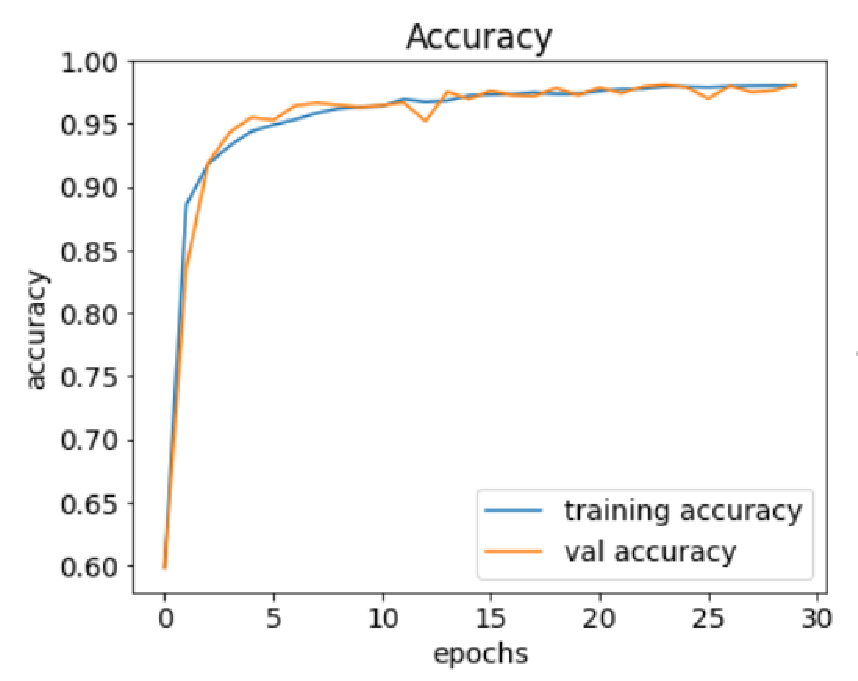
\includegraphics[width=0.7\linewidth]{kennzeichenerkennung/trainingsverlauf.pdf}
    \caption{Verlauf des Modell Trainings}
\end{figure}

Im oberen Bild kann man erkennen, dass die Genauigkeit des Modells bereits nach wenigen Epochen einen Wert von über 90\% erreicht hat und 
nach den 30 Epochen auf einen Endwert von 98,02\% erreicht hat. Das bedeutet, dass bei einem Kennzeichen mit durchschnittlich 7 Zeichen 
eine insgesamte Genauigkeit von 86,93\% erreicht wird. Diese Genauigkeit könnte mit einem längeren Training theoretisch auf einen Wert von 
nahezu 100\% gesteigert werden, aber dazu benötigt es einen stärkeren Computer, welcher zudem noch eine ganze Weile nicht benutzt werden kann.

\subsection{Gehäuse}

\subsubsection{Anforderungen}
Die Anforderungen an das Gehäuse sind recht simpel. Es soll das Modul vor äußeren Einwirkungen schützen, eine Möglichkeit bieten, 
um die Kamera des Raspberry Pi zu befestigen und für weitere Test- und Entwicklungszwecke soll es die wichtigsten Anschlüsse des Raspberry Pi 
zugänglich machen, damit diese verwendet werden können. Zudem sollen die Entwicklungs- und Produktionskosten eher gering sein, weswegen sich ein 
Gehäuse aus dem 3D-Drucker am besten eignet.

\subsubsection{Umsetzung}
Das 3D-Modelling des Gehäuses erfolgte mit dem Programm „Autodesk Fusion 360“/(Fußnote), mit welchem 3D-Modelle erstellt und konvertiert werden können, 
damit man sie mit dem 3D-Drucker ausdrucken kann. In den folgenden Bildern sieht man die Renderansichten der einzelnen Teile.

\begin{figure}[H]
    \centering
    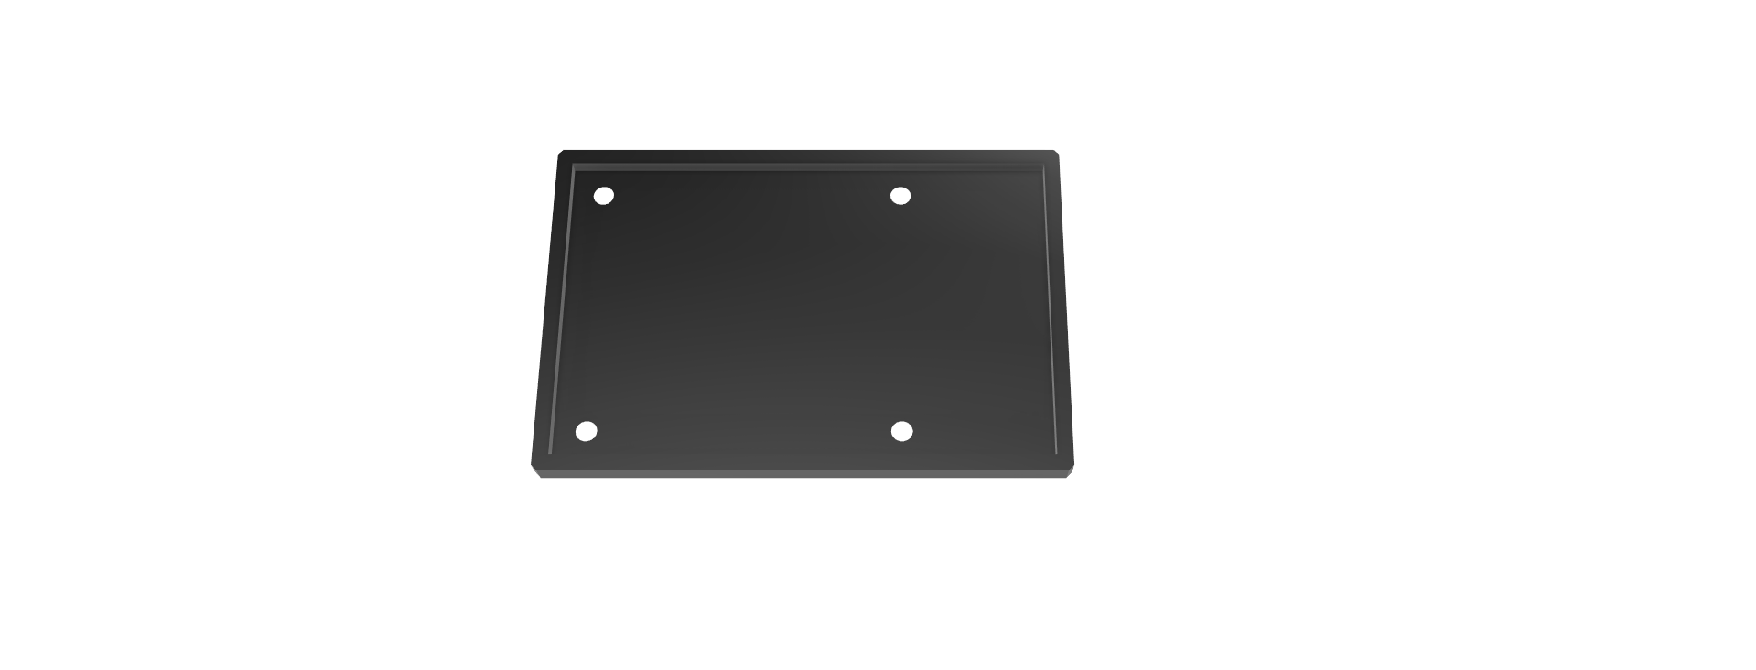
\includegraphics[width=1\linewidth]{kennzeichenerkennung/Renderboden.pdf}
    \caption{Boden des Gehäuses}
\end{figure}

Im ersten Bild sieht man die Renderansicht des Bodens. Auf diesen wird der Raspberry Pi gelegt und mit den 4 Löchern an den mittleren Teil geschraubt. 
Dadurch ist der Raspberry Pi sicher befestigt und kann im Gehäuse nicht verrutschen.

\begin{figure}[H]
    \centering
    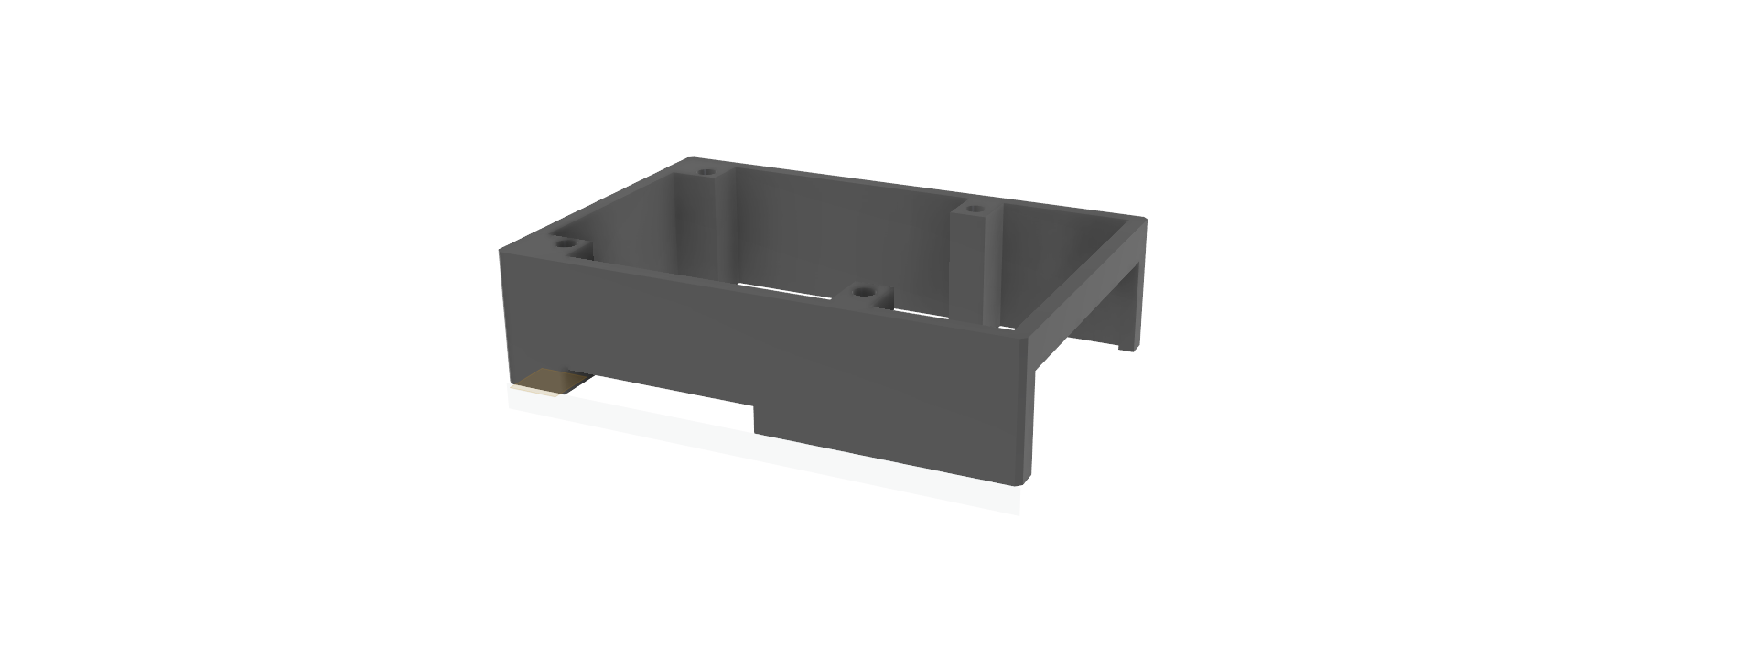
\includegraphics[width=1\linewidth]{kennzeichenerkennung/Rendermittel.pdf}
    \caption{Mittelteil des Gehäuses}
\end{figure}

Der mittlere Teil besitzt 4 Verstärkungen auf der inneren Seite, in welche man Gewinde einfügen kann. Dadurch können der Deckel und der Boden angeschraubt werden. 
Zudem befinden sich auf zwei Seiten Ausschnitte durch welche die Stromversorgung, die HDMI-Ports, die USB-Ports und der Ethernet-Anschluss des Raspberry Pi 
zugänglich sind. Dadurch kann der Raspberry Pi nahezu ohne Einschränkungen mit den wichtigsten Funktionen betrieben werden.

\begin{figure}[H]
    \centering
    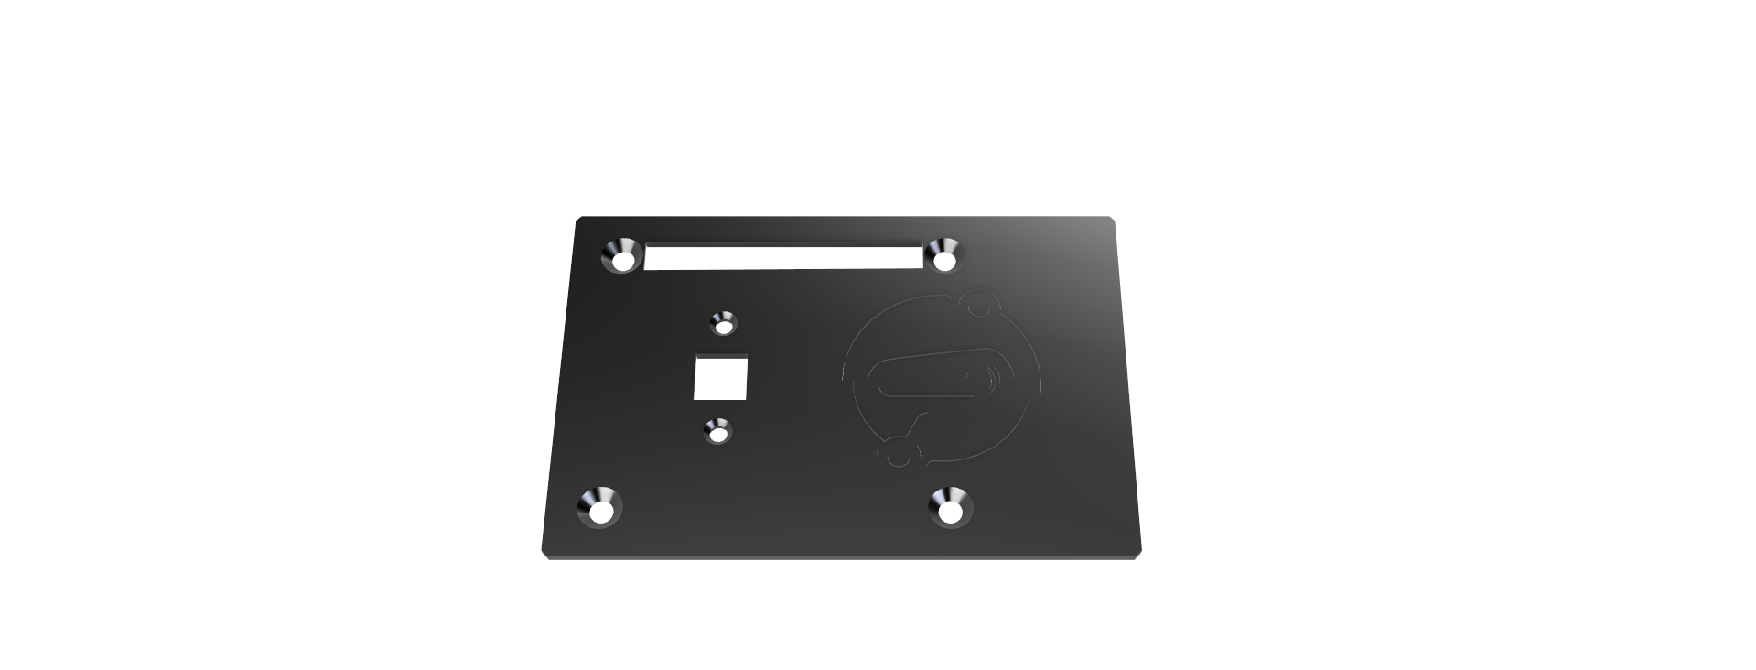
\includegraphics[width=1\linewidth]{kennzeichenerkennung/Renderdeckel.pdf}
    \caption{Deckel des Gehäuses}
\end{figure}

Das letzte Einzelteil ist der Deckel, welcher wieder die gleichen 4 Löcher wie der Boden aufweist, um mit dem Mittelteil verschraubt zu werden. 
Zusätzlich befinden sich im Deckel noch zwei Löcher, um die Kamera festzuschrauben und ein rechteckiges Loch, durch welches die Kamera gesteckt werden kann. 
Außerdem befindet sich auf dem Deckel noch das eingravierte Logo von APM. In der nächsten Abbildung sieht man dann noch eine Gesamtansicht des Gehäuses.

\begin{figure}[H]
    \centering
    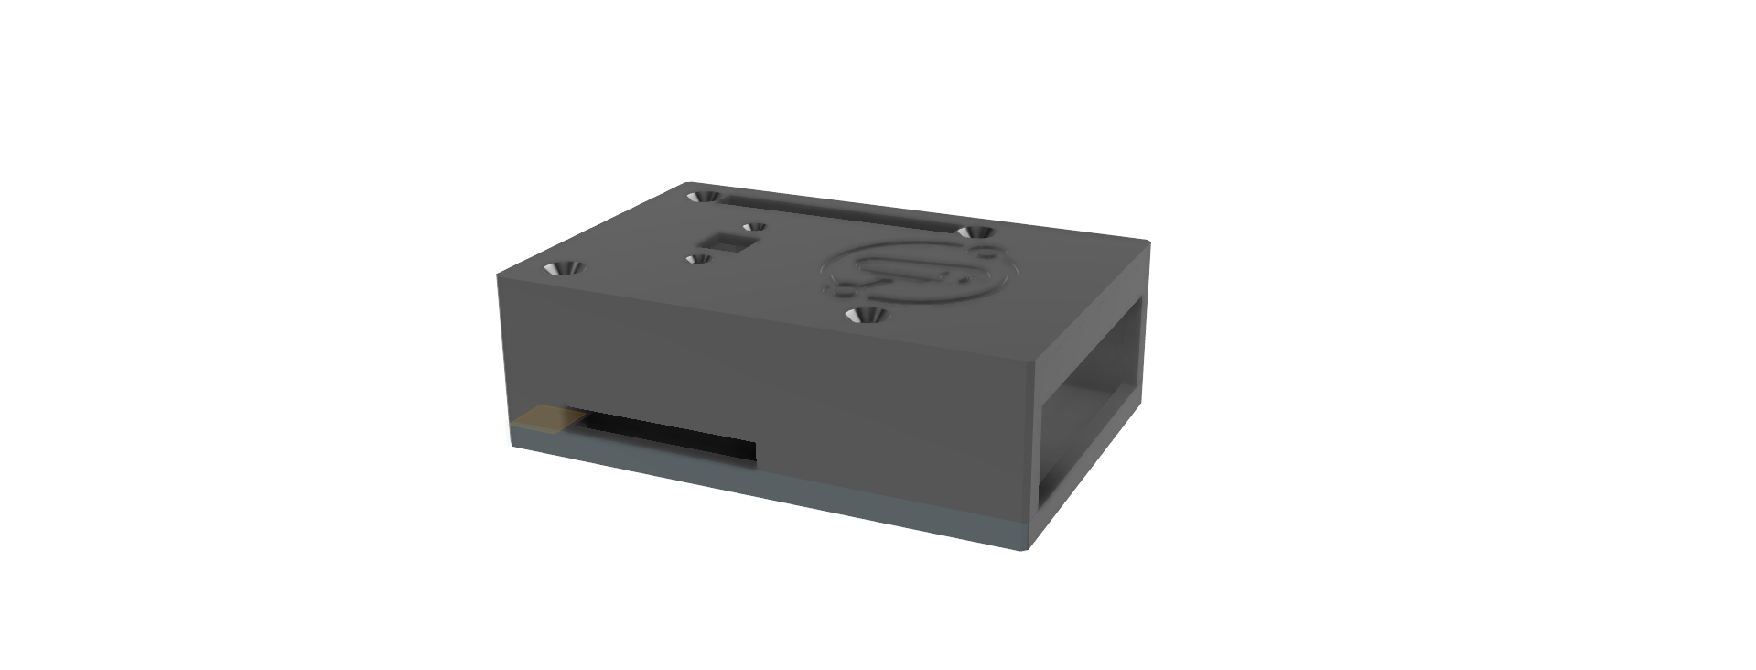
\includegraphics[width=1\linewidth]{kennzeichenerkennung/Rendergesamt.pdf}
    \caption{Gesamtesansicht des Gehäuses}
\end{figure}

Diese Einzelteile wurden dann mit einem 3D-Drucker gefertigt. In den nächsten Bildern sieht man die einzelnen gefertigten Teile und eine Gesamtansicht.

\begin{figure}[H]
    \centering
    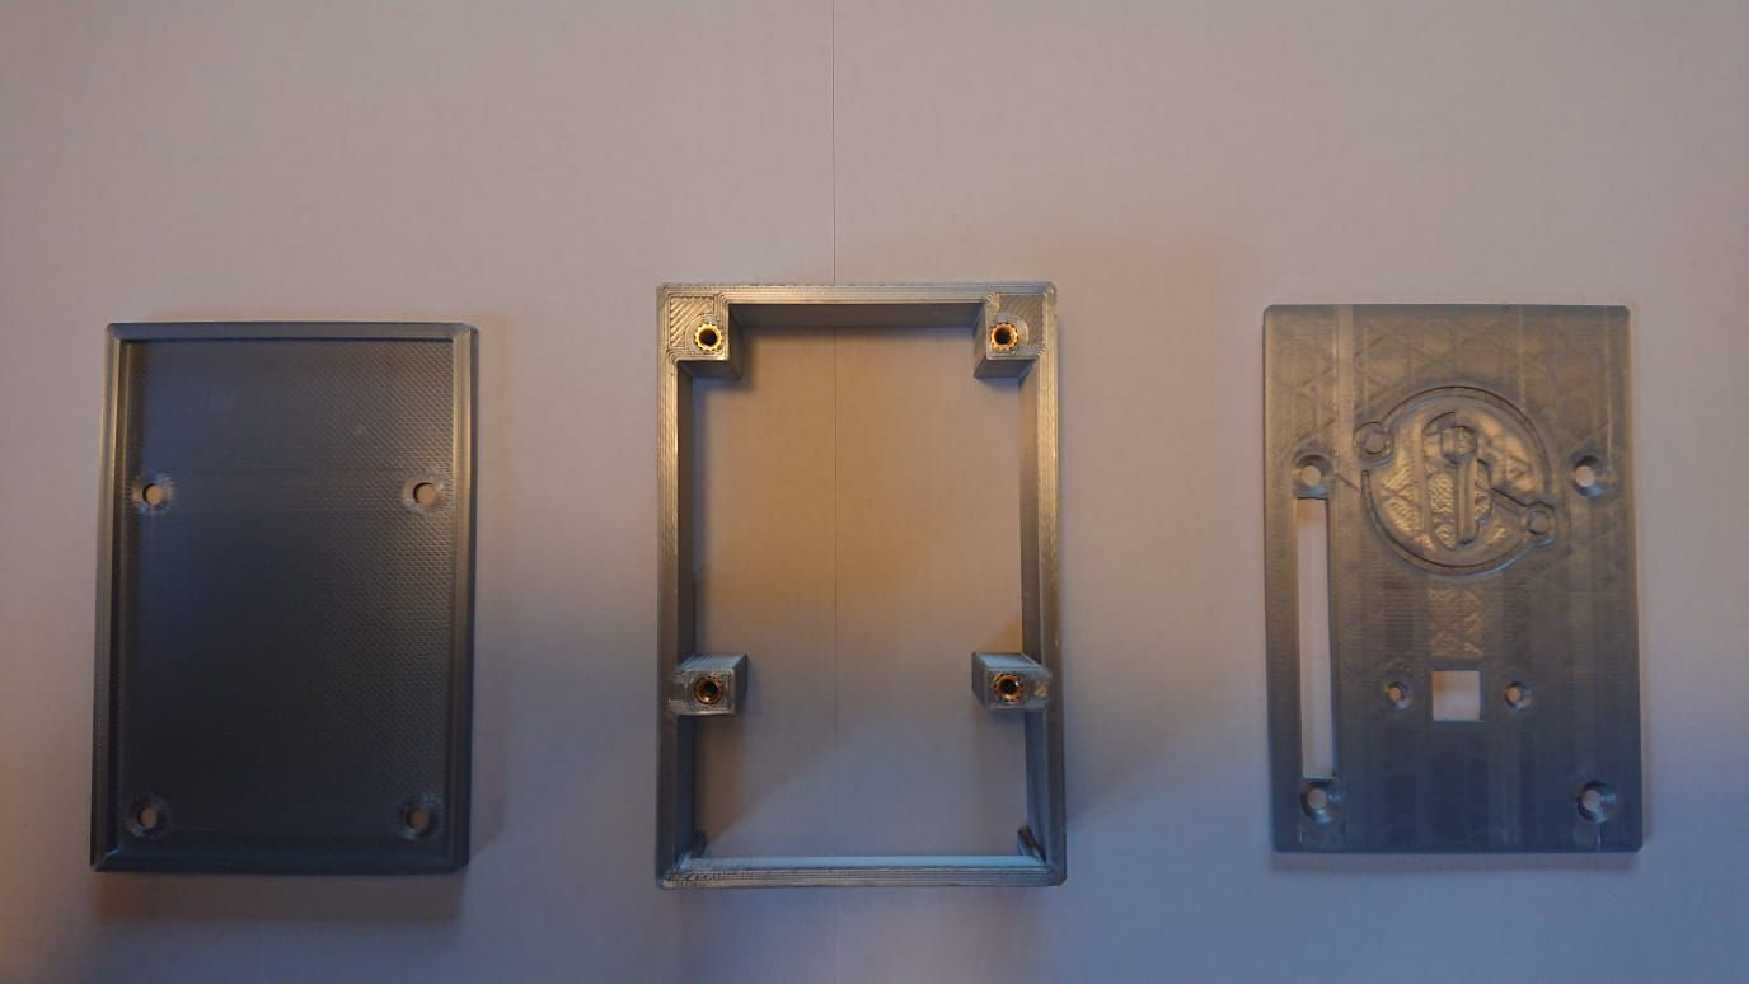
\includegraphics[width=0.8\linewidth]{kennzeichenerkennung/geinzel.pdf}
    \caption{Gedruckte Einzelteile des Gehäuses}
\end{figure}

\begin{figure}[H]
    \centering
    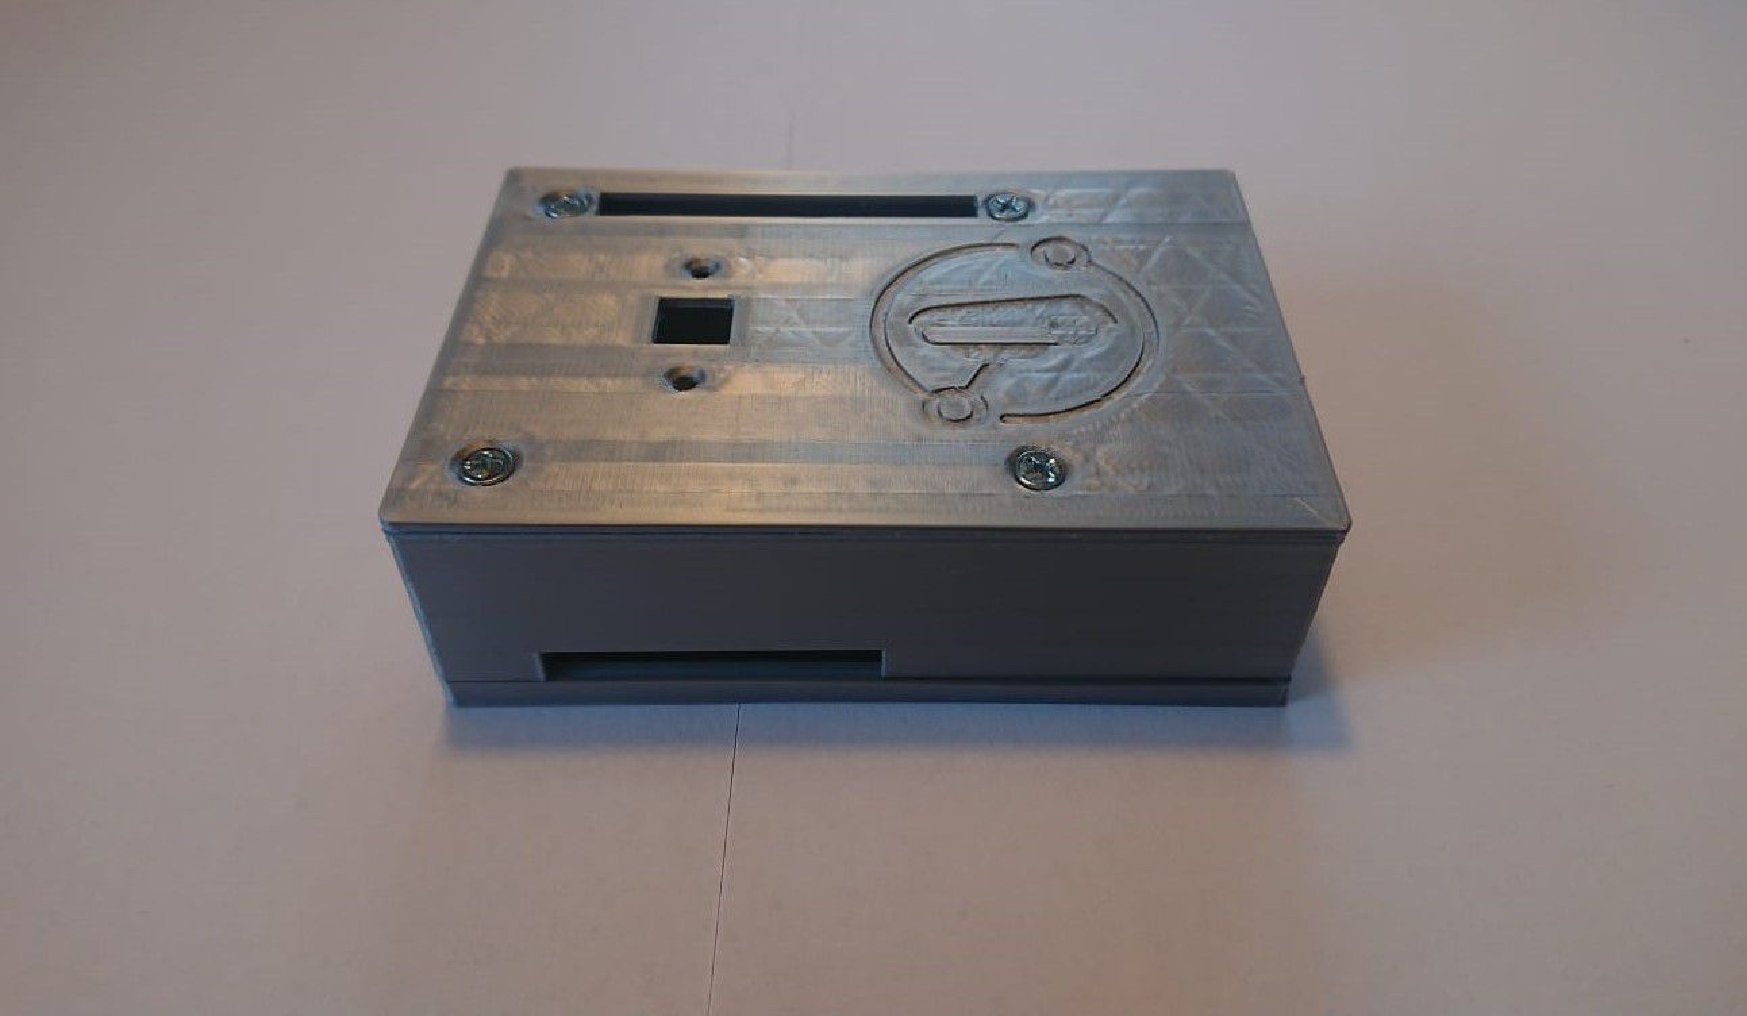
\includegraphics[width=0.8\linewidth]{kennzeichenerkennung/gtogether.pdf}
    \caption{Gesamtesansicht des gedruckten Gehäuses}
\end{figure}

Das fertige Gehäuse erfüllt alle zu Beginn definierten Anforderungen und ist somit bestens für diese Anwendung geeignet.